\documentclass[conference]{IEEEtran}
\IEEEoverridecommandlockouts
\usepackage{cite}
\usepackage{amsmath,amssymb,amsfonts}
\usepackage{graphicx}
\usepackage{textcomp}
\usepackage{xcolor}
\usepackage{booktabs}
\usepackage{tikz}
\usepackage{url}
\usetikzlibrary{arrows.meta,positioning,shapes.geometric,fit,backgrounds,calc}

\newcommand{\TBD}{\textcolor{red}{\textbf{TBD}}}
\newcommand{\silo}{\mathcal{S}}
\newcommand{\onto}{\mathcal{O}}
\newcommand{\rel}{\rho}
\newcommand{\reg}{\mathcal{M}}
\newcommand{\att}{\mathcal{A}}
\newtheorem{proposition}{Proposition}

\def\BibTeX{{\rm B\kern-.05em{\sc i\kern-.025em b}\kern-.08em
    T\kern-.1667em\lower.7ex\hbox{E}\kern-.125emX}}

\begin{document}

\title{FedHarm: A Federated, Closed-Loop Architecture for Ontology\\
Harmonization with Verifier-Stacked Adjudication and Calibrated Abstention}

\author{
    \IEEEauthorblockN{First A. Author\textsuperscript{1}, Second B. Author\textsuperscript{1}, Third C. Author\textsuperscript{2}}
    \IEEEauthorblockA{
        \textsuperscript{1}Department of Computer Science, University Name, City, Country\\
        \textsuperscript{2}Department of Biomedical Informatics, University Name, City, Country\\
        Email: \{first.author, second.author\}@univ.edu, third.author@univ.edu
    }
}

\maketitle

\begin{abstract}
Federated learning (FL) promises collaborative model training without centralizing patient data, but it silently assumes a precondition that healthcare federations rarely satisfy: that each participating site already expresses its records in a vocabulary the others can interpret. Semantic harmonization is therefore the binding constraint on any cross-institutional study, and a recent two-step recipe---embedding-based candidate retrieval followed by large language model (LLM) accept/reject adjudication---demonstrated that the mapping of free-text clinical observations and coded diagnoses onto the MONDO and HPO ontologies can be automated to 78--92\% agreement with a human expert. That architecture, however, is open-loop (accepted mappings are discarded rather than retained), uncalibrated (a hard binary verdict admits no abstention), structure-blind (the ontology is consumed as a bag of labels, so specificity and disjointness errors survive retrieval), and centralized (records are embedded and adjudicated through an external API inside a federation whose premise is that raw data does not move). We propose \emph{FedHarm}, a four-module architecture that inverts each of these properties. \textbf{M1} performs federated hybrid candidate generation: records are embedded at the site, only query vectors cross the boundary, and four complementary generators are unioned with provenance tags. \textbf{M2} interposes an ontology-graph structural verifier that types every candidate by subsumption and disjointness \emph{before} any LLM is invoked, removing the specificity and polarity errors that similarity cannot distinguish. \textbf{M3} replaces the binary oracle with a typed, evidence-citing adjudicator that runs inside the trust boundary under tiered escalation. \textbf{M4} converts adjudicator output into an abstention decision by conformal selection at a target false-discovery rate and writes expert-confirmed mappings into a differentially private \emph{federated mapping registry}, closing the loop so that later rounds and later sites resolve records without new adjudication. We prove four properties of the architecture---pre-filter soundness, finite-sample control of the accepted-set error rate, registry coverage monotonicity, and boundary-independent communication cost. We also consolidate the performance that prior systems have published, across the OAEI Bio-ML alignment benchmark and the record-to-ontology harmonization literature, into two attributed comparison tables, and draw three design consequences from them: accuracy is lost at adjudication rather than at retrieval, reserving the model for borderline cases removes most of its cost without loss of quality, and expert effort rather than model accuracy is the quantity that moves at scale. We then specify a risk--coverage evaluation protocol that measures what a hard accept/reject pipeline cannot: precision at achievable automation coverage, expert-review burden, mapping reuse, cross-site transfer, and privacy--utility trade-off. We also execute the one component that needs no language model---a retrieval pilot over two openly licensed Bio-ML tasks---which tests, and does not support, one of our own pre-registered targets: generator union bought 0.004 and 0.000 recall at 23--45\% additional candidate load. We report no new measurement of the full architecture, and every number we cite for adjudication, calibration, or reuse is attributed to the system that published it. FedHarm preserves the ontology-agnostic, configurable character of the two-step recipe while relocating it inside the trust boundary and adding the uncertainty control that reliable clinical deployment requires.
\end{abstract}

\begin{IEEEkeywords}
federated learning, data harmonization, biomedical ontologies, large language models, selective prediction, conformal risk control, differential privacy
\end{IEEEkeywords}

\section{Introduction}

Federated learning (FL) has become the default answer to the tension between data-hungry model development and the legal and ethical prohibition on moving patient records~\cite{b2,b3,b4,b5}. In the canonical formulation, a coordinator initializes a global model, ships the current parameters to participating sites, receives locally computed updates, and aggregates them into a new global model; raw records never leave institutional boundaries~\cite{b3}. The paradigm has been demonstrated in radiology, oncology, and rare-disease research, and it underpins national and regional health-data infrastructures~\cite{b5,b6}.

The formulation contains an assumption that is easy to overlook. Aggregation of model updates is meaningful only if every site has encoded the same clinical concept in the same way. If one hospital records a pregnancy outcome as the free-text string \emph{``neonatal death''}, a second as ICD-10 code \texttt{P95}, and a third as the SNOMED CT concept for \emph{perinatal death}, then a global model trained over the union is fitting noise: the same label refers to different underlying events at different sites, and different labels to the same event. \emph{Data harmonization}---reconciling heterogeneous types, levels, and sources of data into mutually comparable formats---is consequently not a preprocessing detail but the first precondition of a meaningful federation~\cite{b42,b43}. It is also the step that FL platforms have historically delegated to application-level developers, which is why federated studies remain bespoke artifacts that are rarely reused across consortia~\cite{b1,b43}.

A recent architecture, which we take as our point of departure, showed that harmonization can be substantially automated~\cite{b1,b48}. Its design is a \textbf{two-step pipeline}. In Step~1, candidate pairs are generated for each input record: either by retrieving the $k$ nearest neighbours from a vector index built over ontology labels and synonyms, or by pivoting through cross-references (ICD-10 $\rightarrow$ SNOMED CT $\rightarrow$ MONDO/HPO) harvested from the ontology graphs. In Step~2, an LLM receives each candidate pair together with a natural-language acceptance criterion and returns a binary verdict with a short justification. Evaluated on two real clinical datasets against a single expert physician, the pipeline reached 78--92\% agreement, and the authors drew a clean and generalizable conclusion: retrieval maximizes recall cheaply, and LLM adjudication restores the precision that embedding proximity alone cannot guarantee~\cite{b1}.

That conclusion is correct, and it is the reason the architecture has been influential. Our claim in this paper is narrower and, we believe, more consequential: the two-step design is a \emph{correct decomposition of an incomplete control problem}. Four of its properties are architectural choices rather than incidental implementation details, and each one is a limitation that a different arrangement of the same ingredients removes.

\begin{itemize}
\item \textbf{It is open-loop.} Accepted mappings are emitted and, in the reported system, never retained in a form that benefits the next record, the next study, or the next site. Every deployment re-derives the same correspondences from scratch. The authors themselves identify a shared library of reuseable alignment functions as the natural next step~\cite{b1}.
\item \textbf{It is uncalibrated.} The adjudicator issues a hard accept or reject. There is no calibrated confidence, no abstention band, and therefore no principled way to trade automation coverage against error; a pipeline that is 78\% precise at full coverage cannot be deployed at a fixed risk tolerance, because it cannot concentrate its errors into a reviewable minority.
\item \textbf{It is structure-blind.} The ontology enters as a set of labels and cross-references; its logical axioms are unused. Subsumption and disjointness---the very relations that separate \emph{Grade II} from \emph{$>$grade 2}, or \emph{congenital} from \emph{acquired}---are invisible to a nearest-neighbour search and must be recovered by the LLM from surface form alone. The source study reports this error class explicitly as its dominant residual failure~\cite{b1}.
\item \textbf{It is centralized.} Records are embedded by an external embedding service and adjudicated by an external chat model. The authors flag the contradiction candidly: best-performing models are typically reached through APIs, which conflicts with the data-protection posture of exactly the institutions the federation was built to include~\cite{b1,b45}.
\end{itemize}

\subsection{Contributions}

We propose \textbf{FedHarm}, an architecture that keeps the two-step recipe's generative idea---cheap high-recall generation followed by expensive precision restoration---while changing what is generated, what performs the validation, where the validation runs, and what happens to its output. Our contributions are fivefold.

\textbf{1) A federated, verifier-stacked, closed-loop architecture (Section~\ref{sec:arch}).} FedHarm consists of four modules: federated hybrid candidate generation (M1); an ontology-graph structural verifier that types candidates by subsumption and disjointness before adjudication (M2); a typed LLM adjudicator that returns a relation label, a calibrated confidence, and cited evidence, and that executes inside the trust boundary under tiered escalation (M3); and calibrated abstention coupled to a differentially private federated mapping registry (M4). The registry \emph{closes the loop}: expert-confirmed mappings are retained, aggregated across sites, and re-injected both as a fast-resolution cache and as grounded evidence for future adjudications.

\textbf{2) A formalization of harmonization as selective prediction (Section~\ref{sec:formulation}).} We formulate the task not as a binary decision but as the construction of a \emph{relation-typed, confidence-scored} mapping, and we formulate deployment as choosing an acceptance set that maximizes automation coverage subject to a bounded selective risk. This makes abstention and expert review first-class architectural outputs rather than failure modes.

\textbf{3) Four analytical properties (Section~\ref{sec:analysis}).} We prove that sound structural pre-filtering removes only candidates that cannot satisfy the acceptance relation, so it reduces adjudication volume without recall loss (Proposition~\ref{prop:prefilter}); that conformal selection on the adjudicator's score controls the error rate of the auto-accepted set in finite samples (Proposition~\ref{prop:conformal}); that under accept-only retention the registry's resolution rate is non-decreasing in rounds, so reuse compounds (Proposition~\ref{prop:registry}); and that per-round communication is $O(|\att_i|)$ attestations, independent of local dataset size (Proposition~\ref{prop:comm}). We also characterize the adversarial and privacy surface introduced by a shared mapping artifact.

\textbf{4) A risk--coverage evaluation protocol (Section~\ref{sec:protocol}).} We begin by consolidating the numbers prior systems have actually published---the OAEI Bio-ML alignment benchmark and the record-to-ontology harmonization systems---into two attributed comparison tables (Tables~\ref{tab:oaei} and~\ref{tab:reported}), and show that they jointly establish where the accuracy is lost, that reserving the model for hard cases removes most of its cost, and that expert effort rather than model accuracy is the quantity that moves at scale. We then specify metrics that a hard accept/reject pipeline cannot report---precision at automation coverage, review-burden reduction, registry reuse hit rate, leave-one-site-out transfer, and a privacy--utility accounting---together with six comparison points and a factorial ablation that isolates each module.

\textbf{5) A measured retrieval pilot that disconfirms one of our own targets (Section~\ref{sec:pilot}).} We execute the one component that requires no language model---candidate generation over two openly licensed Bio-ML tasks---and find that a strong lexical generator is not usefully improved by a second generator: union bought 0.004 and 0.000 recall at 23--45\% additional candidate load. We report this against our own pre-registered target rather than around it, and we bound how far it should be read.

We report no new measurement of the full architecture. Every number we cite for adjudication, calibration, or reuse is attributed to the system that published it; the only values in this paper that are ours are those of Table~\ref{tab:pilot}.

\section{Background and Related Work}
\label{sec:related}

\subsection{Federated Learning in Healthcare}

FL replaces data movement with model movement~\cite{b3}. Since the FedAvg formulation, the field has mapped a stable set of open problems: statistical heterogeneity across non-identically distributed site data, systems heterogeneity in compute and availability, privacy accounting under repeated release of updates, and the incentive and governance questions that arise once a consortium is formed~\cite{b2,b4}. Healthcare is the domain where these problems bite hardest, because site data are small, skewed, and governed by statute~\cite{b5}. FedProx and its relatives address heterogeneity by regularizing local objectives toward the global model~\cite{b27}; secure aggregation hides individual updates from the coordinator~\cite{b26}; differentially private training bounds what any single record contributes to a released model~\cite{b24,b25}. Recent work has extended the paradigm to fairness-aware and privacy-preserving collaborative learning~\cite{b6} and to the joint deployment of FL with LLMs~\cite{b36}.

What this literature assumes, almost without exception, is that the label spaces are aligned. When they are not, the failure is silent: aggregation proceeds, a global model is produced, and its semantics are undefined. Harmonization is the missing substrate.

\subsection{Biomedical Ontologies and the Harmonization Problem}

The biomedical domain maintains a dense ecosystem of controlled vocabularies covering diseases, phenotypes, drugs, and procedures~\cite{b7,b8,b9,b10}. SNOMED CT provides a compositional clinical terminology with hierarchical relationships~\cite{b7}; ICD-10 provides the global statistical classification used for reimbursement and public health reporting~\cite{b8}; MONDO unifies disease ontologies from Orphanet, OMIM, and ClinGen~\cite{b9}; HPO standardizes phenotypic abnormality descriptions for genomic diagnostics~\cite{b10}. These vocabularies differ in scope, granularity, and design intent, and the desiderata for a controlled vocabulary---non-vagueness, non-redundancy, non-ambiguity, and consistency of classification and granularity---are precisely the properties that cross-vocabulary mapping threatens~\cite{b11}. Intermediaries such as the UMLS Metathesaurus~\cite{b12} and common data models such as OMOP~\cite{b13} provide partial alignment, and the foundational literature on classification and ontology in precision medicine frames the stakes~\cite{b14}. The practical scale of the effort is documented by national harmonization collaborations, which report that reconciling heterogeneous records across a health system is a substantial, largely manual undertaking~\cite{b49}. Automated ontology matching remains an open problem with its own methodological tradition~\cite{b29}; full automation of clinical harmonization is not available off the shelf~\cite{b1}.

\subsection{LLM-Assisted Harmonization and Its Relatives}

Retrieval-augmented generation established the pattern of grounding a language model's decision in retrieved evidence rather than in parametric memory~\cite{b15}, with dense retrieval as its standard first stage~\cite{b16} and lexical retrieval such as BM25 as its long-standing complement~\cite{b17}. Applied to healthcare interoperability, the pattern has produced LLM-based mapping of clinical text to interchange standards such as FHIR and the US Core Data for Interoperability~\cite{b41,b46,b62}, LLM-assisted harmonization of EHR schemata~\cite{b39}, and concept abstraction frameworks that retrieve top-$k$ candidates and then select among them with a model~\cite{b40}. The two-step architecture of~\cite{b1} sits squarely in this lineage, and predicts---correctly, as the field has since confirmed---that LLMs disrupt entity resolution and schema matching by reasoning beyond surface similarity~\cite{b38}.

A parallel line of work establishes the caution that shapes our design. LLMs are unreliable on complex diagnostic reasoning, and systematic reviews of clinical deployments recommend constraining them to narrow, verifiable roles rather than autonomous generation~\cite{b45,b44}. The source architecture already follows this advice by using the LLM as a binary filter rather than a generative agent~\cite{b1}. FedHarm goes further in the same direction: the LLM is one component of a verifier stack, downstream of a symbolic check and upstream of a calibration layer, and its output is a typed relation with cited evidence rather than a decision.

A partially parallel literature evaluates \emph{ontology matching} rather than record-to-ontology mapping, and it is where the field's only standardized benchmarks live. The OAEI Bio-ML track provides curated reference alignments over OMIM, ORDO, SNOMED CT, FMA, DOID, and NCIT, spanning equivalence and subsumption across five tasks built from MONDO and UMLS cross-references~\cite{b55}. Within it, a clear ordering has emerged. Systems that combine a fast deterministic matcher with LLM prompting reserved for borderline cases now lead the unsupervised setting: MILA attains F1 0.948 on NCIT--DOID and 0.894 on SNOMED--FMA while issuing 92.6--98.4\% fewer LLM requests than a baseline retrieve-then-prompt pipeline~\cite{b54}. Purely LLM-driven refinement fares far worse on the same benchmark---LLMs4OM reaches F1 0.256 on SNOMED--FMA~\cite{b56} and OLaLa reaches 0.649 on OMIM--ORDO~\cite{b57}, against 0.831 for MILA on that task~\cite{b54}---while structure-aware and fine-tuned systems occupy the middle ground~\cite{b58,b59,b61}. Two findings from this line bear directly on our design and are quantified in Section~\ref{sec:prior}. First, candidate generation is not the bottleneck: retrieval recovers up to 100\% of reference mappings, but end-to-end performance drops by as much as 30\% after prompting, and by up to 50\% in the biomedical domain~\cite{b54}. The loss is introduced at adjudication, which is precisely what our M2--M3 ordering is built to prevent. Second, how hierarchy is verbalized matters more than whether it is supplied: phrasing subsumption as ``kind of'' improves recall of hard mappings for smaller reasoning models, whereas the formal ``subclass of'' phrasing degrades it, and some mappings resist every prompt variant tested~\cite{b60}. Both findings argue for making the structural relation explicit and machine-checked rather than leaving the model to infer it from prose. We note that the harmonization literature and the alignment literature have remained largely disjoint---the former does not use the Bio-ML tasks, and the latter does not operate on patient-derived text or under a federation constraint---and that closing this gap in either direction is a contribution we do not attempt here beyond adopting Bio-ML as a second evaluation substrate in Section~\ref{sec:protocol}.

Finally, calibration and selective prediction provide the machinery that the two-step recipe lacks. Modern neural networks are systematically overconfident~\cite{b19}, and the classical remedy is post-hoc scaling or isotonic regression~\cite{b19,b47}. Selective classification formalizes the option to abstain, trading coverage for risk through a rejection threshold~\cite{b20,b21}. Conformal prediction and its risk-controlling extension supply distribution-free, finite-sample guarantees on the selected set under exchangeability~\cite{b23,b50,b22}. We use conformal risk control as the M4 decision rule precisely because it converts an uncalibrated LLM score into a bound that a clinical review board can act on.

\subsection{Positioning}

FedHarm shares with~\cite{b1} the problem, the domain, the ontology-agnostic and prompt-configurable character of the acceptance criteria, and the division of labour between recall-oriented generation and precision-oriented validation. It differs in four respects, summarized in Table~\ref{tab:delta}. The comparison is architectural: it concerns which components exist, where they execute, what they emit, and what is retained, not the choice of embedding model or ontology.

\begin{table}[t]
\caption{Architectural delta between the two-step pipeline of~\cite{b1} and FedHarm.}
\label{tab:delta}
\centering
\footnotesize
\begin{tabular}{@{}p{1.75cm}p{2.75cm}p{2.9cm}@{}}
\toprule
\textbf{Dimension} & \textbf{Two-step pipeline~\cite{b1}} & \textbf{FedHarm} \\
\midrule
Stages & 2: retrieve, adjudicate & 4: retrieve, verify, adjudicate, calibrate \\
Ontology role & Label and synonym bag; cross-refs & Logical graph with axioms; subsumption and disjointness \\
Candidate sources & Dense retrieval \emph{or} cross-ref pivot & Four generators unioned with provenance \\
LLM output & Binary verdict + justification & Relation type + confidence + cited evidence \\
LLM locus & External API & In-boundary, tiered escalation \\
Uncertainty & None (hard decision) & Conformal abstention, routed review \\
Retained artifact & None & DP federated mapping registry \\
Federated scope & Model weights & Model weights \emph{and} the harmonization artifact \\
Precision from & LLM alone & Symbolic check, LLM, and calibration \\
\bottomrule
\end{tabular}
\end{table}

The FL infrastructure context is unchanged. FedHarm is designed to be instantiated inside programmable federation frameworks such as Vantage6~\cite{b34}, Brane~\cite{b33}, and the EPI platform~\cite{b35}, all of which already solve containerized remote execution, policy enforcement, and orchestration, and all of which leave data alignment to the application.

\section{Problem Formulation}
\label{sec:formulation}

\subsection{Setting}

Let there be $N$ sites $\silo_1,\dots,\silo_N$, site $i$ holding a local dataset $D_i$ of records that must not leave $\silo_i$. Let $\onto$ be a target ontology with term set $\mathcal{T}$, label function $\ell : \mathcal{T} \to \Sigma^{*}$, and logical axioms interpretable by a description-logic reasoner. Let $\mathcal{R}$ be a set of alignment relations,
\begin{equation}
\mathcal{R} = \{\equiv,\ \sqsupseteq,\ \sqsubseteq,\ \bot,\ \sim\},
\end{equation}
denoting respectively equivalence, the target being broader than the source, the target being narrower, disjointness, and unspecified relatedness. Harmonization is the construction, for each record $x \in D_i$, of a set of relation-typed mappings
\begin{equation}
h(x) \subseteq \mathcal{T} \times \mathcal{R},
\end{equation}
and the deployment contract is an \emph{acceptance policy} $\pi$ that commits to some of these mappings and defers the rest.

The two-step pipeline of~\cite{b1} instantiates $\mathcal{R}$ implicitly with $|\mathcal{R}| = 2$ (accept, reject) and returns a single commitment per candidate with no deferral. We make the relation explicit because it is what the acceptance criterion actually depends on---a fact the source authors discovered empirically when they had to clarify their criterion from ``same condition'' to ``same \emph{or more generic}'' mid-study~\cite{b1}.

\subsection{Target Ontologies Are Graphs, Not Bags}

For $c_1, c_2 \in \mathcal{T}$, write $c_1 \sqsubseteq c_2$ when $\onto \models \forall z.\ c_1(z) \rightarrow c_2(z)$. A reasoner answers subsumption, equivalence, and disjointness queries over $\onto$; for EL and Horn fragments, which cover the majority of biomedical ontologies, this is tractable in polynomial time~\cite{b31}, and OWL~2 reasoners such as HermiT provide the general case~\cite{b30,b32}. Throughout, we assume the reasoner is \emph{sound}: if it returns $c_1 \sqsubseteq \neg c_2$, then $c_1$ and $c_2$ are in fact disjoint. Soundness is the standard guarantee for these systems and is the only property Proposition~\ref{prop:prefilter} requires.

\subsection{Selective Prediction}

Let $s(x,c) \in [0,1]$ be a score such that larger values indicate a more confident commitment, computed by whatever stack of verifiers the architecture assembles. For a threshold $\tau$, define the acceptance set
\begin{equation}
\att_\tau = \{(x,c) : s(x,c) \ge \tau\}
\end{equation}
and the selective risk
\begin{equation}
\mathrm{risk}(\tau) = \mathbb{E}\!\left[\, \ell\big(h(x,c),\, y(x,c)\big) \;\middle|\; (x,c) \in \att_\tau \right],
\end{equation}
where $\ell$ is a task loss and $y$ the ground-truth relation. Coverage is $\mathrm{cov}(\tau) = \Pr[(x,c) \in \att_\tau]$. The deployment requirement is
\begin{equation}
\text{maximize } \mathrm{cov}(\tau) \quad \text{subject to} \quad \mathrm{risk}(\tau) \le \epsilon ,
\label{eq:objective}
\end{equation}
for a risk tolerance $\epsilon$ set by the study's review board. Equation~\eqref{eq:objective} is the objective the two-step pipeline cannot express, because with a hard decision $\tau$ is effectively $0$ and coverage is fixed at $1$.

\subsection{The Federated Constraint}

We require that no record text, no label, and no embedding of a record cross a site boundary. What may cross are (i) query \emph{vectors} derived from local records, optionally noised; (ii) attestations of accepted mappings, i.e.\ pairs in $\mathcal{T} \times \mathcal{R}$ with provenance metadata; and (iii) model parameters, in the classical FL sense, when the architecture is co-deployed with a training loop.

\section{The FedHarm Architecture}
\label{sec:arch}

\subsection{Overview}

FedHarm replaces the retrieve-then-adjudicate pair with a four-stage verifier stack whose stages are ordered by cost and by the kind of evidence they consume: a cheap broad stage that cannot be confidently wrong because it commits to nothing, a symbolic stage that is exact within its fragment, an expensive stage that reasons over surface meaning, and a statistical stage that decides what to commit. Fig.~\ref{fig:arch} shows the arrangement.

\begin{figure*}[t]
\centering
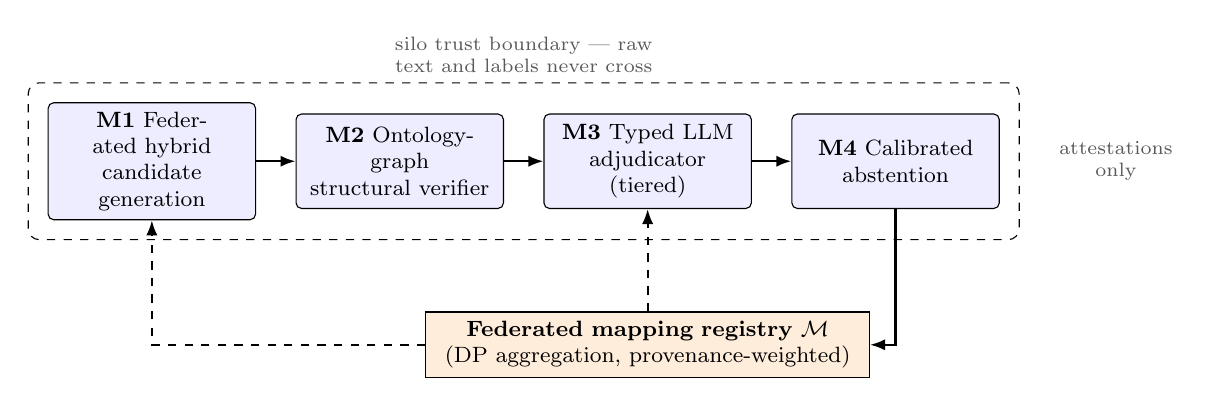
\begin{tikzpicture}[font=\footnotesize,>=Latex,
  mod/.style={draw,rounded corners=2pt,align=center,text width=2.4cm,minimum height=1.2cm,fill=blue!7},
  store/.style={draw,align=center,text width=5.4cm,minimum height=0.75cm,fill=orange!14},
  arr/.style={-{Latex[length=1.9mm]},thick},
  darr/.style={-{Latex[length=1.9mm]},thick,dashed}]
\node[mod] (m1) {\textbf{M1} Federated hybrid\\candidate generation};
\node[mod,right=5mm of m1] (m2) {\textbf{M2} Ontology-graph\\structural verifier};
\node[mod,right=5mm of m2] (m3) {\textbf{M3} Typed LLM\\adjudicator (tiered)};
\node[mod,right=5mm of m3] (m4) {\textbf{M4} Calibrated\\abstention};
\draw[arr] (m1) -- (m2);
\draw[arr] (m2) -- (m3);
\draw[arr] (m3) -- (m4);
\node[store,below=13mm of m3] (reg) {\textbf{Federated mapping registry} $\reg$ \ (DP aggregation, provenance-weighted)};
\draw[arr] (m4.south) |- (reg.east);
\draw[darr] (reg.north) -- (m3.south);
\draw[darr] (reg.west) -| (m1.south);
\begin{scope}[on background layer]
\node[draw,dashed,rounded corners,inner sep=7pt,fit=(m1)(m2)(m3)(m4),
      label={[font=\scriptsize,text=black!65,text width=6.2cm,align=center]above:silo trust boundary --- raw text and labels never cross}] (bound) {};
\end{scope}
\node[font=\scriptsize,align=center,text=black!65,right=4mm of m4,text width=1.9cm] {attestations\\only};
\end{tikzpicture}
\caption{The FedHarm pipeline. Records are embedded locally in M1; only query vectors reach the shared ontology index. M2 types candidates by subsumption and disjointness before any model call. M3 adjudicates residual ambiguity inside the boundary and emits a typed relation with cited evidence. M4 sets the commit set by conformal selection and writes expert-confirmed mappings to the registry, which feeds back into both M1 (fast resolution) and M3 (grounded exemplars), closing the loop.}
\label{fig:arch}
\end{figure*}

\subsection{M1: Federated Hybrid Candidate Generation}

M1 produces, for each record $x$ at site $i$, a candidate set that is deliberately over-inclusive, because M2--M4 only ever remove candidates. Let $G = \{g_{\mathrm{dense}}, g_{\mathrm{lex}}, g_{\mathrm{graph}}, g_{\mathrm{xref}}\}$ be four generators, each returning a ranked list. Then
\begin{equation}
C(x) = \bigcup_{g \in G} C_g(x), \qquad
C_g(x) = \mathrm{top}\text{-}k_g\big(\mathrm{rank}_g(x)\big),
\end{equation}
and each candidate $c$ carries a provenance tag $\mathrm{src}(c) \subseteq G$ recording which generators proposed it.

\begin{itemize}
\item \textbf{Dense retrieval} ($g_{\mathrm{dense}}$) over a shared index of ontology labels and synonyms, using a sentence encoder~\cite{b18}. The record is encoded at the site; the resulting vector, optionally clipped and noised, is the only object that leaves.
\item \textbf{Lexical retrieval} ($g_{\mathrm{lex}}$) with BM25 over the same index~\cite{b17}. Lexical matching recovers exact-terminology hits that dense encoders blur, and it is the generator whose behaviour is stable under distribution shift.
\item \textbf{Graph expansion} ($g_{\mathrm{graph}}$) takes the top lexical and dense hits as anchors and adds their ancestors, descendants, and siblings within a bounded radius $r$ in $\onto$. This is the generator that converts a near-miss into a hit: if the true target is an ancestor of a retrieved term, retrieval alone will never surface it, but one-hop expansion will.
\item \textbf{Cross-reference pivoting} ($g_{\mathrm{xref}}$) follows harvested cross-references through an intermediary vocabulary, as in the ICD-10 $\rightarrow$ SNOMED CT $\rightarrow$ MONDO/HPO path of~\cite{b1}, and is the only generator that applies when input records are already coded.
\end{itemize}

The union is the design decision that matters most in principle. The source study found the two generators it used to be complementary rather than interchangeable---only a minority of input codes were matched by both, and neither achieved coverage alone~\cite{b1}. Trending the candidate set from union toward intersection would convert that finding from a reported observation into an architectural invariant. We flag at once that our own retrieval pilot on curated alignment tasks does not support union over a strong lexical generator (Section~\ref{sec:pilot}), and we return to why that null result may not transfer from curated terminologies to free clinical text.

\subsection{M2: Ontology-Graph Structural Verifier}

M2 is a symbolic stage that consumes the candidate set and types each candidate against an anchor $a(x)$, namely the ontology term already known or most confidently resolved for $x$ (for coded inputs, the term reached through cross-references; for free text, the highest-scoring lexical-dense agreement). It issues reasoner queries to assign
\begin{equation}
\rel\big(a(x), c\big) \in \{\equiv,\ \sqsupseteq,\ \sqsubseteq,\ \bot,\ \sim\},
\end{equation}
where $\bot$ is returned when $\onto \models c \sqsubseteq \neg a(x)$, and $\sim$ is the residual label when the reasoner can assert neither subsumption nor disjointness. Alongside the relation, M2 emits the \emph{specificity direction} (whether $c$ is more generic, more specific, or incomparable) and the axiom path that justified it, which M3 receives as evidence.

Two effects follow. First, candidates typed $\bot$ are eliminated with certainty: a term disjoint from the anchor can never satisfy an equivalence, broader-than, or narrower-than criterion, so removing it is lossless for any acceptance relation drawn from $\{\equiv, \sqsupseteq, \sqsubseteq\}$ (Proposition~\ref{prop:prefilter}). Second, for candidates that survive, M3 is no longer asked to infer the relation from strings; it is asked to \emph{confirm or refute} a relation that the ontology already asserts or refutes. This is the direct remedy for the dominant residual error class of the two-step pipeline, whose failures are overwhelmingly specificity and polarity confusions---\emph{Grade II} against \emph{$>$grade 2}, \emph{congenital} against \emph{acquired}, \emph{APGAR at minute 1} against \emph{10-minute APGAR}~\cite{b1}---that a reasoner settles exactly and a nearest-neighbour search cannot see at all.

Two independent results support putting this stage first. MILA's retrieve--identify--prompt design converges on the same principle from the ontology-alignment side, reserving model calls for the cases its search cannot resolve, and reports a 92.6--98.4\% reduction in LLM requests without loss of quality~\cite{b54}; Proposition~\ref{prop:prefilter} supplies a sufficient condition under which a reduction of that kind is available at no cost in recall. And the benchmark evidence that LLM-only refinement collapses in the biomedical domain---F1 0.256 for LLMs4OM on SNOMED--FMA against 0.894 for a matcher-first system on the same task~\cite{b56,b54}---argues that a structure-aware stage is a prerequisite rather than an optimization. We note the important asymmetry: MILA's structural signal comes from a matcher over labels, whereas M2's comes from the ontology's logical axioms, so the two are complementary rather than equivalent.

\subsection{M3: Typed LLM Adjudicator}

M3 handles the candidates that are not settled symbolically: those typed $\sim$, and those whose structural relation must be checked against the record's surface meaning. Its contract differs from the binary oracle in three ways.

\textbf{Typed output.} The adjudicator returns a structured verdict
\begin{equation}
\big(\hat{r},\ \hat{p},\ \mathcal{E},\ j\big),
\end{equation}
where $\hat{r} \in \mathcal{R}$ is the predicted relation, $\hat{p} \in [0,1]$ a self-reported confidence, $\mathcal{E}$ the evidence items M3 actually relied on (the M2 axiom path, the matching label or synonym, the record span), and $j$ a bounded justification. Requiring evidence citations does two things: it makes the verdict auditable by a reviewer who sees the same evidence, and it supplies the feature signal that M4 calibrates.

\textbf{In-boundary execution with tiered escalation.} The adjudicator runs on a locally hosted open-weight model, so the record text never leaves the site. A small local model resolves the high-agreement majority; a larger local model, invoked only when the small model's score falls in the indeterminate band or when M2 returned $\sim$ with a conflicting direction, resolves the residual. Escalation is decided by the score, not by a fixed schedule, so cost tracks difficulty. This is the architecture's answer to the privacy contradiction the source authors raise: the accuracy benefits of a strong validator are retained, but the validator is inside the federation~\cite{b1,b25}.

\textbf{Prompt-configurable criteria.} As in~\cite{b1}, the acceptance criterion is natural language, so switching from equivalence to subsumption---or from ``same or more generic'' to ``same or more specific''---is a configuration change and not a code change. FedHarm preserves this property and adds a machine-readable relation label, so the criterion becomes a policy over $\mathcal{R}$ rather than a sentence the model must interpret unaided.

\subsection{M4: Calibrated Abstention and the Federated Mapping Registry}

M4 is the stage that turns per-candidate verdicts into a committed mapping and, critically, into a retained one.

\textbf{Score construction and calibration.} The raw confidence $\hat{p}$ is not usable as a decision score: self-reported LLM confidences are miscalibrated and typically overconfident~\cite{b19,b28}. M4 therefore fits a calibration map $\phi$ on a small per-site labeled calibration set, using temperature scaling or isotonic regression~\cite{b19,b47}, and forms
\begin{equation}
s(x,c) = \phi\big(\hat{p}(x,c)\big),
\end{equation}
optionally augmented with structural agreement between $\hat{r}$ and $\rel(a(x),c)$.

\textbf{Conformal risk control.} Rather than fixing $\tau$ by a grid search against a validation split, M4 selects the largest threshold whose calibration-set selective risk satisfies the tolerance, using conformal risk control with a monotone loss~\cite{b22,b23}. This yields the finite-sample guarantee of Proposition~\ref{prop:conformal} and directly implements the constrained objective of Eq.~\eqref{eq:objective}: coverage is maximized subject to risk, and the abstained residual is exactly the review queue.

\textbf{The registry.} Expert decisions on the abstained residual, together with high-confidence auto-accepted mappings, are written as \emph{attestations}
\begin{equation}
\alpha = \big(c_{\text{src}},\ c_{\text{tgt}},\ r,\ s,\ \mathrm{prov}\big),
\end{equation}
into the federated mapping registry $\reg$. The registry is aggregated across sites rather than merged blindly: attestation support is counted, weighted by provenance trust and by the calibration quality of the contributing site, and the published aggregate is noised and suppressed below a support threshold $k_{\min}$ so that a mapping attested by fewer than $k_{\min}$ independent sites is not disclosed. This is the point at which the architecture introduces a genuine federated learning problem over the harmonization artifact itself, distinct from---and complementary to---FL over model weights~\cite{b24,b25,b26}. Because a registry entry can leak the presence of a rare local term at a site, the support threshold and noise scale are part of the disclosure policy, not an afterthought; we return to this in Section~\ref{sec:analysis}.

\textbf{Closing the loop.} The registry feeds back in two distinct ways, shown in Fig.~\ref{fig:loop}. As a \emph{cache}, an attestation resolves a future occurrence of the same source term directly, at negligible cost, and short-circuits M1--M3. As \emph{grounding}, attested mappings from other sites are retrieved and injected into the M3 context as confirmed precedents, which raises adjudication accuracy for the residual cases that the cache does not cover. The loop is what makes the architecture cumulative: unlike the two-step pipeline, whose output is terminal, FedHarm's output is the next round's input.

\begin{figure}[t]
\centering
\resizebox{\columnwidth}{!}{%
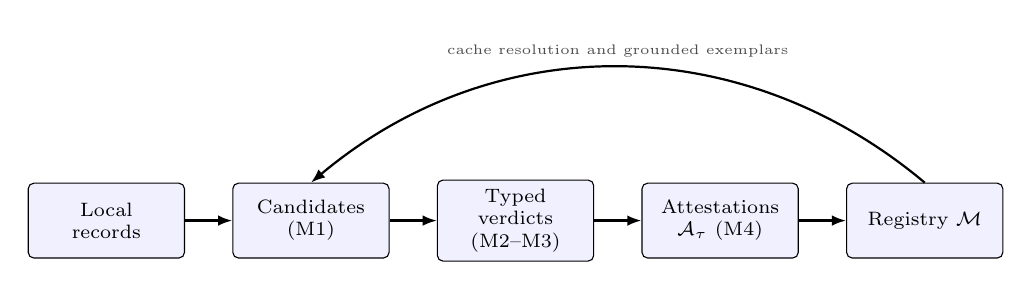
\begin{tikzpicture}[font=\scriptsize,>=Latex,node distance=6mm,
  n/.style={draw,rounded corners=2pt,align=center,text width=1.75cm,minimum height=0.95cm,fill=blue!6},
  arr/.style={-{Latex[length=1.8mm]},thick}]
\node[n] (a) {Local\\records};
\node[n,right=of a] (b) {Candidates\\(M1)};
\node[n,right=of b] (c) {Typed\\
verdicts (M2--M3)};
\node[n,right=of c] (d) {Attestations\\$\att_\tau$ (M4)};
\node[n,right=of d] (e) {Registry $\reg$};
\draw[arr] (a)--(b); \draw[arr] (b)--(c); \draw[arr] (c)--(d); \draw[arr] (d)--(e);
\draw[arr] (e.north) to[out=140,in=40] node[above,font=\tiny,text=black!70,pos=0.5]{cache resolution and grounded exemplars} (b.north);
\end{tikzpicture}}
\caption{The closed loop. Attestations accumulate into a shared registry; the registry both resolves records directly and supplies confirmed precedents to the adjudicator, so coverage compounds across rounds and sites.}
\label{fig:loop}
\end{figure}

\subsection{Operating Modes}

Three modes make the architecture adoptable incrementally. In \emph{assisted} mode M4 auto-accepts nothing and the pipeline is a review-queue generator, which is the closest analogue to a purely human workflow. In \emph{supervised} mode, the default, M4 auto-accepts above $\tau$ and routes the residual to experts while the registry accumulates. In \emph{autonomous} mode, enabled only after the registry has saturated for the ontology pair in question, unattested records fall through to M1--M4 but the majority resolve from the registry. Because the risk bound is a function of the calibration set, not of the mode, moving between modes is a change of $\epsilon$ in Eq.~\eqref{eq:objective} rather than a change of architecture.

\section{Evaluation Protocol}
\label{sec:protocol}

We specify the protocol because the architecture's claims are claims about a trade-off curve, and a curve has to be measured at more than one point.

\subsection{Datasets and Splits}

The reference setting is the one established by~\cite{b1}, which is drawn from the maternal and pediatric therapeutics context of the MPRINT hub~\cite{b37}: a set of unannotated clinical observations spanning pregnancy exposures and outcomes to be mapped to MONDO and HPO, and a set of ICD-10-coded outcomes to be mapped to the same ontologies through an intermediate vocabulary. To exercise the federated claims, records must be partitioned across simulated sites along a realistic axis---by institution of origin, or, where origin is unavailable, by a stratification that induces label-space heterogeneity, so that different sites observe different concept frequencies. Calibration, registry construction, and evaluation splits must be disjoint; the registry is never populated from the evaluation split.

We add a second, standardized substrate that the harmonization literature has not used. The OAEI Bio-ML track supplies curated reference alignments over five ontology pairs---OMIM--ORDO, NCIT--DOID, SNOMED--FMA, and two SNOMED--NCIT tasks---with published baselines spanning logic-based, fine-tuned, and LLM-refined systems (Table~\ref{tab:oaei})~\cite{b55,b54}. Running FedHarm on Bio-ML has two benefits. It makes the architecture directly comparable to a mature literature under a shared reference alignment rather than to a single expert's judgment, and it isolates the contribution of M2, because Bio-ML's ontology pairs differ sharply in how much structural information they expose: aligning SNOMED--FMA exercises subsumption heavily, whereas NCIT--DOID is largely lexical. A verifier stack that helps only on structurally rich pairs should be visible as a task-dependent effect, and we treat that as a falsifiable prediction rather than a hypothesis. The record-to-ontology setting remains the primary evaluation, since it is the task a federation actually confronts; Bio-ML is a controlled complement, and we report the two separately rather than pooling them.

\subsection{Reported Performance of Prior Systems}
\label{sec:prior}

Before specifying what to measure, we record what has already been measured, because the numbers determine which comparisons are meaningful. Two distinct task families are involved, and conflating them is a common error. \emph{Ontology-to-ontology alignment} matches concepts of one ontology against another and is evaluated against curated reference alignments; \emph{record-to-ontology harmonization} maps patient-derived strings or codes onto ontology terms and is evaluated against expert judgment. FedHarm addresses the second, but the first supplies the only standardized benchmark in the area, and its measurements are directly informative about where a verifier stack should intervene.

Table~\ref{tab:oaei} reports the unsupervised results on the OAEI Bio-ML track~\cite{b55}, the machine-learning-friendly biomedical benchmark whose five tasks are built from MONDO and UMLS cross-references. Table~\ref{tab:reported} reports the record-to-ontology systems, which use heterogeneous metrics and are therefore not directly comparable to one another.

\begin{table*}[t]
\caption{Reported performance on the OAEI Bio-ML biomedical ontology-alignment benchmark, unsupervised setting. All values are as published by the original systems and as compiled in~\cite{b54}; none is measured by us. Task difficulty varies widely: OMIM--ORDO is the hardest and NCIT--DOID the easiest.}
\label{tab:oaei}
\centering
\footnotesize
\begin{tabular}{@{}llrrrl@{}}
\toprule
\textbf{System} & \textbf{Task} & \textbf{Precision} & \textbf{Recall} & \textbf{F1} & \textbf{Method family} \\
\midrule
LogMap~\cite{b59}         & OMIM--ORDO            & 0.876 & 0.448 & 0.593 & Logic-based, structure-aware \\
LogMap~\cite{b59}         & NCIT--DOID            & 0.934 & 0.668 & 0.779 & Logic-based, structure-aware \\
BERTMap~\cite{b58}        & OMIM--ORDO            & 0.734 & 0.576 & 0.646 & Fine-tuned encoder \\
BERTMap~\cite{b58}        & NCIT--DOID            & 0.888 & 0.878 & 0.883 & Fine-tuned encoder \\
SORBETMatcher~\cite{b61}  & NCIT--DOID            & 0.920 & 0.907 & 0.913 & Fine-tuned Siamese encoder \\
OLaLa~\cite{b57}          & OMIM--ORDO            & 0.735 & 0.582 & 0.649 & LLM refinement \\
LLMs4OM~\cite{b56}        & OMIM--ORDO            & 0.718 & 0.580 & 0.641 & LLM refinement \\
LLMs4OM~\cite{b56}        & SNOMED--FMA           & 0.211 & 0.326 & 0.256 & LLM refinement (collapses) \\
\midrule
MILA~\cite{b54}           & OMIM--ORDO            & 0.879 & 0.778 & 0.831 & Matcher + LLM for borderline cases \\
MILA~\cite{b54}           & NCIT--DOID            & 0.964 & 0.932 & 0.948 & Matcher + LLM for borderline cases \\
MILA~\cite{b54}           & SNOMED--FMA           & 0.964 & 0.834 & 0.894 & Matcher + LLM for borderline cases \\
MILA~\cite{b54}           & SNOMED--NCIT (Pharm)  & 0.981 & 0.772 & 0.864 & Matcher + LLM for borderline cases \\
MILA~\cite{b54}           & SNOMED--NCIT (Neopl)  & 0.928 & 0.880 & 0.903 & Matcher + LLM for borderline cases \\
\bottomrule
\end{tabular}
\end{table*}

\begin{table*}[t]
\caption{Reported performance of record-to-ontology harmonization systems. Metrics are heterogeneous across rows (expert agreement, accuracy, F1, time reduction) and rows are comparable only within a metric. All values are as published by the cited systems; the final row is our proposed architecture, which is not yet measured and for which we claim no number.}
\label{tab:reported}
\centering
\footnotesize
\begin{tabular}{@{}llll@{}}
\toprule
\textbf{System} & \textbf{Task} & \textbf{Metric} & \textbf{Reported value} \\
\midrule
Kokash et al.~\cite{b1} & MPRINT ICD-10 $\rightarrow$ MONDO/HPO, RAG candidates & Expert agreement & 0.78 \\
Kokash et al.~\cite{b1} & MPRINT ICD-10 $\rightarrow$ MONDO/HPO, SNOMED pivot & Expert agreement & 0.91 \\
Kokash et al.~\cite{b1} & MPRINT unannotated outcomes $\rightarrow$ MONDO/HPO & Expert agreement & 0.92 \\
Kokash et al.~\cite{b1} & Candidate acceptance rate (RAG / SNOMED) & Accepted fraction & 0.423 / 0.147 \\
EHRmonize, GPT-4o 10-shot~\cite{b40} & Medication route abstraction (MIMIC-IV, eICU) & Accuracy & 0.97 \\
EHRmonize, GPT-4o 10-shot~\cite{b40} & Generic drug name extraction & Accuracy & 0.82 \\
EHRmonize, GPT-4o 10-shot~\cite{b40} & Antibiotic binary classification & F1 & 1.00 \\
EHRmonize~\cite{b40} & Annotation time versus fully manual review & Reduction & 60.4--67.9\% \\
MILA~\cite{b54} & LLM requests versus baseline retrieve-then-prompt & Reduction & 92.6--98.4\% \\
\midrule
FedHarm (this work) & Record-to-ontology harmonization, federated & --- & not measured \\
\bottomrule
\end{tabular}
\end{table*}

Three conclusions follow, and each one is load-bearing for the design of Sections~\ref{sec:arch} and \ref{sec:protocol}.

\textbf{(i) Adjudication, not retrieval, is where the accuracy is lost.} On the Bio-ML benchmark, candidate retrieval recovers up to 100\% of the reference mappings, yet end-to-end performance falls by up to 30\% after prompting---and by up to 50\% in the biomedical domain, where LLM-based refinement performs worst~\cite{b54}. The SNOMED--FMA row of Table~\ref{tab:oaei} is the clearest instance: a purely LLM-refined system reaches F1 0.256~\cite{b56} where a matcher-plus-borderline-LLM system reaches 0.894 on the same task~\cite{b54}. A pipeline that treats the language model as the sole arbiter is therefore not merely imprecise; it discards most of the recall its own retriever achieved. This is the empirical case for interposing a symbolic stage ahead of adjudication (M2), and it is the reason we treat the LLM as one component of a verifier stack rather than as the validator.

\textbf{(ii) Reserving the model for hard cases preserves quality and removes most of the cost.} MILA's retrieve--identify--prompt design makes exactly this move from the alignment side and reports a 92.6--98.4\% reduction in LLM requests relative to a baseline retrieve-then-prompt pipeline, while leading four of five tasks~\cite{b54}. Proposition~\ref{prop:prefilter} supplies the reason a reduction of this kind is available without a corresponding loss of recall. The source harmonization pipeline does not exploit it, because its adjudicator is invoked on every candidate all four of its generators produce.

\textbf{(iii) Expert effort, not model accuracy, is the quantity that moves at scale.} EHRmonize reduces annotation time by 60.4--67.9\% relative to manual labeling while retaining clinician oversight, and reports its residual corrections as a small, enumerable set~\cite{b40}. This is direct precedent for treating review burden as a first-class reported quantity rather than an implementation detail, and it is why Section~\ref{sec:protocol} measures coverage at a fixed error tolerance instead of accuracy at full coverage. The harmonization systems of Table~\ref{tab:reported} report a single operating point; the alignment systems of Table~\ref{tab:oaei} report precision, recall, and F1 at full coverage. Neither reports a risk--coverage curve, and consequently neither states the error rate a deployment would actually incur at a chosen level of automation.

\subsection{Baselines and Ablations}

\begin{itemize}
\item \textbf{B1, retrieval only.} The candidate generators of M1 with no validation, i.e.\ the source pipeline's Step~1~\cite{b1}. Establishes the recall ceiling.
\item \textbf{B2, two-step pipeline.} M1 plus a binary LLM adjudicator with the published prompt~\cite{b1}. The direct comparison.
\item \textbf{B3, union retrieval + binary LLM.} B2 with the multi-generator union of M1, isolating the contribution of candidate breadth from the contribution of the verifier stack.
\item \textbf{B4, FedHarm without M2.} Full pipeline minus the structural verifier, isolating symbolic contribution.
\item \textbf{B5, FedHarm without M4 calibration.} Abstention by raw self-reported confidence and a fixed threshold, isolating the calibration contribution.
\item \textbf{B6, FedHarm without the registry.} The loop opened, isolating reuse.
\end{itemize}
The full architecture is evaluated in all three operating modes. A factorial ablation over \{M2 on/off\} $\times$ \{M4 on/off\} $\times$ \{registry on/off\} separates main effects from interactions, which matters because the source study found harness components to interact non-additively---an individual edit can help in isolation and regress in combination---and we expect the same of a verifier stack~\cite{b1}.

\subsection{Metrics}

\begin{itemize}
\item \textbf{Mapping quality.} Precision, recall, and F1 of committed mappings, computed separately per relation class, since a pipeline that is reliable for $\equiv$ may be unreliable for $\sqsubseteq$.
\item \textbf{Risk--coverage.} The curve $\mathrm{cov}(\tau) \mapsto \mathrm{risk}(\tau)$, summarized by the area under the risk--coverage curve and by precision at fixed coverage levels (50\%, 70\%, 90\%). This is the primary metric; a scalar precision at full coverage, as reported by the two-step pipeline, is the $\mathrm{cov}=1$ endpoint of the curve and the least informative point on it.
\item \textbf{Automation coverage at risk tolerance.} The largest coverage satisfying the error-rate bound for $\epsilon \in \{0.05, 0.10, 0.20\}$: for FedHarm, the accepted-set size under the Benjamini--Hochberg rule of Proposition~\ref{prop:conformal} together with the empirical false discovery rate against the nominal $\epsilon$; for threshold baselines, the largest $\mathrm{cov}(\tau)$ with $\mathrm{risk}(\tau) \le \epsilon$. The gap between nominal and empirical error rate is reported as a separate column, since it is the direct test of the calibration stage.
\item \textbf{Review burden.} Fraction of candidates routed to expert review under M4, against the all-candidates review baseline; reported per site. EHRmonize's 60.4--67.9\% annotation-time reduction under mandatory clinician oversight is the closest published precedent and sets the bar this metric should be compared against~\cite{b40}, with the caveat that time reduction and candidate-review fraction are different quantities and we report both.
\item \textbf{Reuse and transfer.} Registry hit rate over rounds; share of a site's records resolved by a cache whose entries were attested at \emph{other} sites, i.e.\ cross-site harmonization transfer.
\item \textbf{Privacy--utility.} Mapping quality and registry hit rate as functions of the privacy budget and support threshold, with the guarantee certified by an accounting method appropriate to the noising scheme~\cite{b24}.
\item \textbf{Cost.} Adjudicator invocations per record, tier-1 versus tier-2 split, and wall-clock and token cost per committed mapping, so that the symbolic stage's savings are quantified rather than asserted.
\end{itemize}

\subsection{Expert Protocol and Statistical Analysis}

The source study evaluated agreement against a single expert, a design it correctly identifies as a limitation, and it further showed that a single expert's judgments shift when the acceptance criterion is clarified~\cite{b1}. We therefore specify a panel of at least three clinical reviewers with disjoint subsets and a shared subset for inter-annotator agreement, with the relation criterion fixed in writing before annotation begins. Agreement is reported as Cohen's $\kappa$ or Krippendorff's $\alpha$ among experts, and expert--architecture agreement is reported against the majority verdict with the panel's disagreement rate as a ceiling. Comparisons across baselines use paired bootstrap resampling over records with confidence intervals; because the baselines share candidates, a paired design is both more powerful and more honest than comparing marginal accuracies.

\subsection{Reporting Format and Published Baselines}

Table~\ref{tab:results} fixes the reporting format and pre-populates the two baseline rows with the source study's published values, so that the comparison anchor is stated rather than implied~\cite{b1}. Everything a reviewer would have to take on trust is confined to the baseline block and is marked as such; no cell in the rows we are responsible for is estimated.

\begin{table*}[t]
\caption{Evaluation table for FedHarm. The B1--B2 rows reproduce values published by the source study~\cite{b1} and are \emph{not} our measurements; the remaining rows are to be produced by the protocol of this section and are reported as empty rather than estimated. ``---'' denotes a quantity the source does not report. Precision for B2 is the expert-agreement rate, which that study also reports as mapping precision.}
\label{tab:results}
\centering
\footnotesize
\begin{tabular}{@{}llrrrrr@{}}
\toprule
\textbf{Method} & \textbf{Candidate generation} & \textbf{Precision} & \textbf{Recall} & \textbf{Coverage at $\epsilon$} & \textbf{Emp.\ FDR} & \textbf{Reuse} \\
\midrule
\multicolumn{7}{@{}l}{\textit{Prior systems --- values as published by~\cite{b1}, not measured by us}} \\
B1 Retrieval only~\cite{b1}     & RAG, $k{=}3$      & --- & 0.98\textsuperscript{a} & --- & --- & --- \\
B1 Retrieval only~\cite{b1}     & SNOMED pivot      & --- & 0.688\textsuperscript{b} & --- & --- & --- \\
B2 Two-step pipeline~\cite{b1}  & RAG, $k{=}3$      & 0.78 & --- & --- & --- & 0.00 \\
B2 Two-step pipeline~\cite{b1}  & SNOMED pivot      & 0.91 & --- & --- & --- & 0.00 \\
B2 Two-step pipeline~\cite{b1}  & Unannotated, $k{=}3$ & 0.92 & --- & --- & --- & 0.00 \\
\midrule
\multicolumn{7}{@{}l}{\textit{Our systems --- to be produced by the protocol of Section~\ref{sec:protocol}}} \\
B3 Union + binary LLM           & union of four generators & \TBD & \TBD & \TBD & \TBD & 0.00 \\
B4 FedHarm without M2           & union, no structural verifier & \TBD & \TBD & \TBD & \TBD & \TBD \\
B5 FedHarm without calibration  & union, M2, uncalibrated LLM & \TBD & \TBD & \TBD & \TBD & \TBD \\
B6 FedHarm without registry     & full, loop open & \TBD & \TBD & \TBD & \TBD & 0.00 \\
FedHarm (supervised)            & full pipeline & \TBD & \TBD & \TBD & \TBD & \TBD \\
FedHarm (autonomous)            & full, saturated registry & \TBD & \TBD & \TBD & \TBD & \TBD \\
\bottomrule
\end{tabular}

\smallskip
{\footnotesize \textsuperscript{a}Ceiling the source reports would be attainable by expanding retrieval to $k{=}10$ (98\% of entries); it is not a measured end-to-end recall. \textsuperscript{b}Derived by us from a published count: 800 of 1{,}162 ICD-10 codes yielded at least one candidate.}
\end{table*}

\subsection{Pre-registered Targets and Their Anchors}
\label{sec:targets}

Because we cannot fill the rows we are responsible for, we state in advance what would count as success, and we anchor every target to a number published by another system rather than to a value chosen for convenience. Table~\ref{tab:targets} is the numeric companion to Table~\ref{tab:results}: it supplies the quantity that each empty cell must be measured against. Every value in its third column is another system's published result, never ours.

\begin{table}[t]
\caption{Pre-registered targets for FedHarm and the published results that anchor them. The anchor column reports other systems' measurements, not ours. ``---'' means no published analogue exists, which is itself the novelty claim for M4's registry: no system in either literature retains harmonization output.}
\label{tab:targets}
\centering
\footnotesize
\begin{tabular}{@{}p{0.72cm}p{2.15cm}p{3.63cm}@{}}
\toprule
\textbf{ID} & \textbf{Target for FedHarm} & \textbf{Anchoring published result} \\
\midrule
T1 & $\ge$80\% fewer adjudicator calls than B3 & 92.6--98.4\% fewer LLM requests than a baseline retrieve-then-prompt pipeline on OAEI~\cite{b54} \\
T2 & FDR $\le$ 0.10 at coverage $\ge$ 0.70 & Source commits to 100\% of candidates at precision 0.78--0.92, i.e.\ 8--22\% error~\cite{b1} \\
T3 & B3 recall exceeds B2 recall & \emph{Tested; not supported}---union gained 0.004 and 0.000 recall on two Bio-ML tasks at 23--45\% more candidates~\cite{b1} \\
T4 & B4 FDR rises in specificity and polarity classes & LLM-only refinement F1 0.256 versus 0.894 matcher-first, SNOMED--FMA~\cite{b56,b54} \\
T5 & Review fraction $\le$ 0.30 against 1.00 & 60.4--67.9\% annotation-time reduction with clinician oversight retained~\cite{b40} \\
T6 & Registry reuse $\ge$ 0.40 by round three & ---\ (no published analogue; monotonicity from Proposition~\ref{prop:registry}) \\
\bottomrule
\end{tabular}
\end{table}

Two targets are falsifiable in a strong sense. T3 fails if generator union does not raise recall above the single-generator baseline, which would deny that the complementarity the source study reports matters architecturally; it was testable without a language model, and the pilot of Section~\ref{sec:pilot} does not support it. T4 fails if disabling the structural verifier does not concentrate new errors in the specificity and polarity classes, which would mean the benefit of M2 lies somewhere other than the error classes we claim for it. Table~\ref{tab:targets} is a commitment about comparison, not a forecast: we do not predict what FedHarm will score, and filling Table~\ref{tab:results} with projections derived from this column would be reporting a model of a model.

\section{Analytical Properties}
\label{sec:analysis}

The architecture makes four claims that hold independently of any experiment.

\begin{proposition}[Structural pre-filtering is lossless for the acceptance relation]
\label{prop:prefilter}
Let $\mathcal{R}^{+} \subseteq \{\equiv, \sqsupseteq, \sqsubseteq\}$ be the set of relations the acceptance criterion admits, let $C(x)$ be the candidate set, and let $\tilde{C}(x) = \{c \in C(x) : \rel(a(x),c) \neq \bot\}$ be the set surviving M2, where $\rel$ is computed by a sound reasoner. Then no candidate whose true relation to the anchor lies in $\mathcal{R}^{+}$ is removed, and $|\tilde{C}(x)| \le |C(x)|$, with equality if and only if no candidate is disjoint from the anchor.
\end{proposition}

\noindent\textit{Proof.} Suppose $\rel(a(x),c) = \bot$, so $\onto \models c \sqsubseteq \neg a(x)$. Since $a(x)$ and $c$ are satisfiable ontology terms, it follows that $c$ is disjoint from $a(x)$, hence can be neither equivalent to it, nor broader, nor narrower than it. The true relation of $c$ therefore cannot lie in $\mathcal{R}^{+}$, so removal discards no admissible candidate. The cardinality claim is immediate. \hfill$\square$

The proposition is what licenses placing a cheap exact stage before an expensive approximate one: M2 can only reduce the adjudication volume, and it reduces it precisely on the candidates whose apparent similarity is coincidental.

\begin{proposition}[Finite-sample control of the accepted-set error rate]
\label{prop:conformal}
For a candidate $(x,c)$ let $H(x,c)$ be the null hypothesis that its true relation does not lie in $\mathcal{R}^{+}$, and let $p(x,c) \in (0,1]$ be a conformal p-value for $H(x,c)$ computed against a calibration set exchangeable with the test population~\cite{b50,b52}. Let $\att_\epsilon$ be the set of candidates selected by the Benjamini--Hochberg rule at level $\epsilon$ applied to the test p-values. Then
\begin{equation}
\mathrm{FDR}(\att_\epsilon)
\;=\;
\mathbb{E}\!\left[
\frac{\big|\{(x,c) \in \att_\epsilon : H(x,c)\ \text{holds}\}\big|}{\max\{|\att_\epsilon|,1\}}
\right]
\;\le\; \epsilon ,
\end{equation}
and, under independence of the p-values, $\att_\epsilon$ is the largest threshold rule satisfying that bound.
\end{proposition}

\noindent\textit{Proof.} Conformal p-values are super-uniform under the null whenever calibration and test candidates are exchangeable~\cite{b50}, which is exactly the validity condition the Benjamini--Hochberg procedure requires. The procedure's theorem then yields $\mathrm{FDR} \le \epsilon$ for positively dependent p-values and, under independence, identifies it as the largest threshold set with that property~\cite{b53}. \hfill$\square$

Proposition~\ref{prop:conformal} is the formal content of the claim that M4 converts an uncalibrated model score into a deployable contract, and it explains why the source pipeline's reported precision range is not directly actionable: a precision figure without a coverage figure and a calibrated score is a single point on an unmeasured curve. Two qualifications belong in the statement rather than in a footnote. First, the controlled quantity is the false discovery rate, that is, the error rate of the accepted set averaged over selections; if a bound on the expected fraction of errors over \emph{all} candidates is preferred instead, the conformal risk control construction of~\cite{b22} applies, at the cost of a less directly interpretable operating point. Second, the guarantee is distribution-free but not assumption-free, because it requires exchangeability---a condition a site with a different coding practice may violate. A hard accept/reject pipeline reports neither quantity.

\begin{proposition}[Registry coverage is monotone under accept-only retention]
\label{prop:registry}
Let $\reg_t$ be the registry after round $t$, and let $R_t$ be the fraction of records resolved directly from $\reg_t$. If the retention rule is accept-only---an attestation, once published, is never revoked or overwritten---and registry lookup is deterministic, then $R_t \le R_{t+1}$ for all $t$.
\end{proposition}

\noindent\textit{Proof.} Accept-only retention gives $\reg_t \subseteq \reg_{t+1}$, so the set of source terms for which a registry entry exists grows. The resolved set satisfies $\{x : \reg_t(x) \neq \bot\} \subseteq \{x : \reg_{t+1}(x) \neq \bot\}$, whence $R_t \le R_{t+1}$. \hfill$\square$

The proposition holds under accept-only retention and is exactly what revocation, provenance decay, or DP suppression below $k_{\min}$ can violate; we state the condition rather than the unconditional claim for that reason. Its practical reading is that the loop, when it is stable, is monotonically cumulative, so the amortized cost of harmonization falls with consortium size and study duration---the property that turns a reusable library from an aspiration into an architectural consequence.

\begin{proposition}[Boundary-independent communication cost]
\label{prop:comm}
Per round, site $i$ transmits $|\att_i|$ attestations of constant size, so the architecture's communication is $O\!\left(\sum_i |\att_i|\right)$, independent of $|D_i|$, of the number of records adjudicated, and of any embedding dimension used inside the boundary.
\end{proposition}

\noindent\textit{Proof.} The only objects crossing the boundary are query vectors---fixed-length, independent of $|D_i|$---and attestations, each a tuple of two ontology identifiers, a relation label, a scalar score, and provenance metadata. Registries are broadcast once and cached. No term proportional to local dataset size or record length appears in either direction. \hfill$\square$

This is the property that makes the architecture a federated one in the strict sense rather than a distributed one: the boundary traffic is a function of the \emph{harmonization artifact}, not of the data being harmonized.

\subsection{Privacy and Adversarial Surface of the Registry}

Introducing a shared artifact introduces a shared attack surface, and we treat it as part of the architecture rather than a caveat. Two risks are material.

\textbf{Inference from attestations.} A published mapping from a rare local term to an ontology code can reveal that a site holds at least one record containing that term. The standard mitigations are the ones we build in: the support threshold $k_{\min}$ suppresses mappings attested by too few independent sites, and noise calibrated to a budget bounds the per-attestation disclosure~\cite{b24,b25}. Because the registry is queried many times over a study's life, the composition of these releases must be accounted for, not just the privacy of a single release.

\textbf{Poisoning by a participating site.} A malicious or merely broken site can attest mappings that are wrong, and a naive majority rule over a small consortium can be swayed by one adversarial participant. The architecture's defences are structural rather than heroic: provenance-weighted aggregation down-weights sites whose attestations are later contradicted by expert review, and robust aggregation rules developed for Byzantine-tolerant federated learning---trimmed means and distance-based filtering---apply directly to attestation aggregation because the object being aggregated is a finite multiset of labels with numeric scores~\cite{b51}. We note also that the adversarial surface is smaller than it first appears: M2 remains sound regardless of what any site attests, so a poisoned registry can degrade the cache but cannot make a disjoint candidate acceptable, and the conformal guarantee is computed over the site's own calibration set rather than over the registry.

\subsection{Where the Architecture Can Still Fail}

Three failure modes are foreseeable and should be measured rather than argued away. First, if the anchor $a(x)$ used in M2 is itself wrong---which is the case when the record is unannotated and the top lexical-dense agreement is mistaken---then structural typing propagates the error, and the pre-filter is no longer lossless with respect to the \emph{true} relation. M2's soundness is relative to the anchor, and the protocol must therefore report anchor accuracy separately. Second, the conformal guarantee requires exchangeability between calibration and test, which a new site with a different coding practice violates; the guarantee then holds only conditionally, and coverage should be re-estimated per site. Third, a registry that saturates on easy concepts can entrench a wrong mapping that was attested early and never revisited; accept-only retention, which gives Proposition~\ref{prop:registry}, is the mechanism that permits this, and a controlled revocation policy is the price of correcting it.

\section{Measured Pilot on Bio-ML}
\label{sec:pilot}

\begin{figure*}[t]
\centering
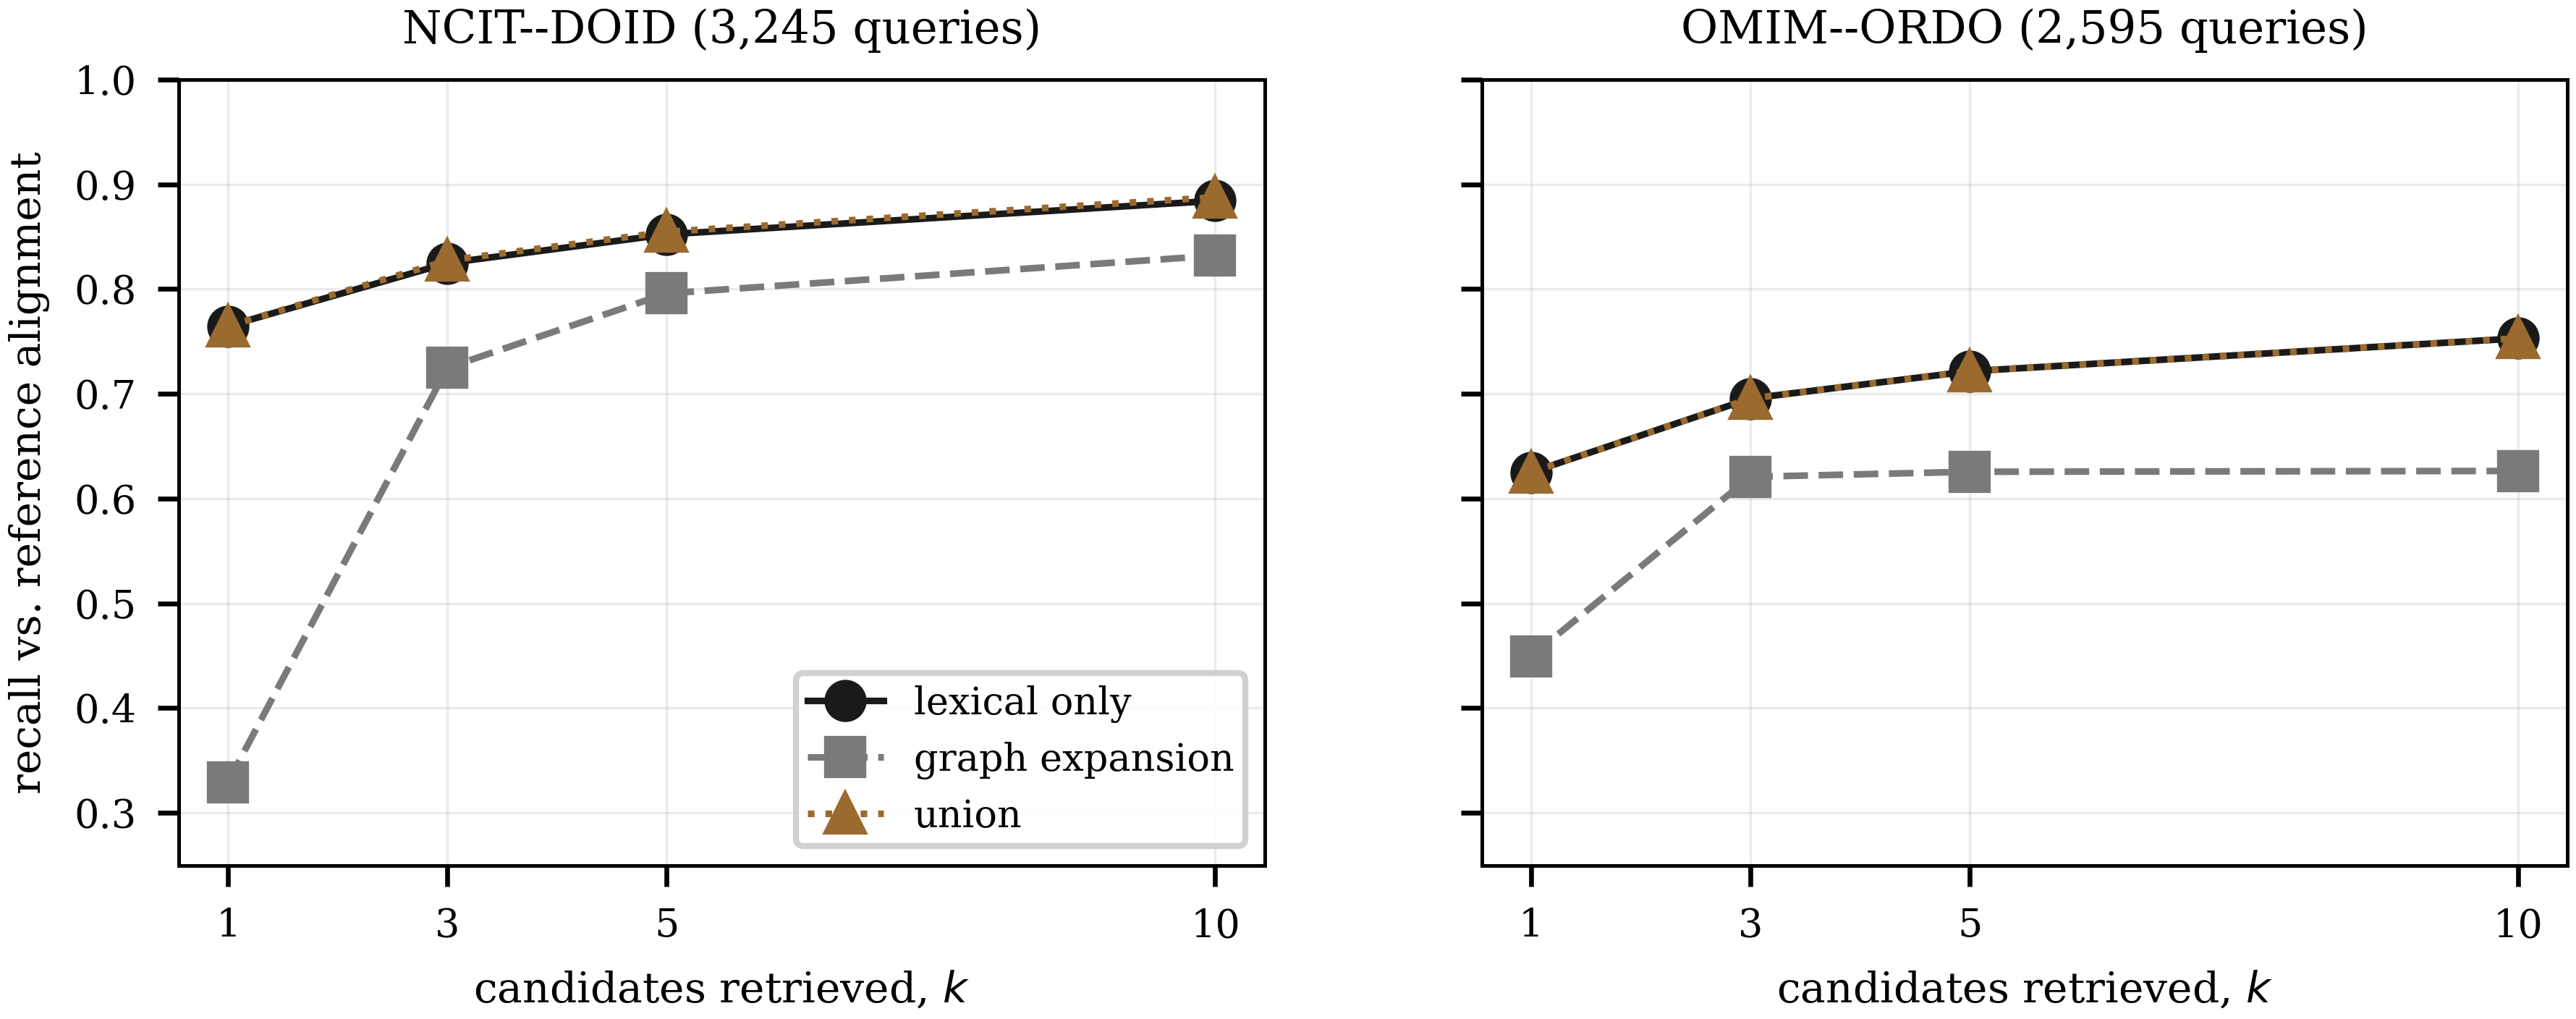
\includegraphics[width=\textwidth]{figs/fig_recall_k.png}
\caption{Recall against number of retrieved candidates, measured on the two openly licensed Bio-ML tasks. The union curve is visually coincident with the lexical curve at every $k$ on both tasks, which is the negative result reported below: adding the graph generator changes recall by at most 0.004 while inflating the candidate set by 23--45\%. On OMIM--ORDO the graph generator is the weakest of the three throughout.}
\label{fig:recallk}
\end{figure*}

The only component of FedHarm that can be executed without a language model is M1, and we report the result although it is unfavourable to one of our own pre-registered predictions. The pilot covers the two Bio-ML tasks whose ontologies are openly licensed---NCIT--DOID and OMIM--ORDO---and excludes the three SNOMED-based tasks, which require a licence we do not hold. It implements one of M1's four generators: BM25 lexical retrieval over target labels and synonyms, evaluated against the reference equivalence alignments. A second generator that expands the asserted class hierarchy around the leading lexical anchors is implemented in two variants, one bounded to parents and children of the top anchor and one expanding siblings from the top three anchors. Dense retrieval requires an encoder that was not available, and cross-reference pivoting requires SNOMED CT. Adjudication (M3), calibration, and the registry (M4) are therefore absent from the pilot, so no row of Table~\ref{tab:results} is filled by it and no M3 or M4 claim is tested.

\begin{table*}[t]
\caption{Measured retrieval pilot on the OAEI Bio-ML benchmark. Values are our own measurements against the reference equivalence alignments; candidate counts are means over queries. The union row is the bounded expansion variant, which is the more favourable of the two we tried.}
\label{tab:pilot}
\centering
\footnotesize
\begin{tabular}{@{}llrrrr@{}}
\toprule
\textbf{Task (\#queries)} & \textbf{Generator} & \textbf{P} & \textbf{R} & \textbf{F1} & \textbf{Cand.} \\
\midrule
NCIT--DOID (3{,}245) & lexical, $k{=}1$  & 0.769 & 0.765 & 0.766 & 9.0 \\
NCIT--DOID           & lexical, $k{=}10$ & 0.148 & 0.884 & 0.221 & 9.0 \\
NCIT--DOID           & graph, $k{=}10$   & 0.324 & 0.829 & 0.451 & 4.2 \\
NCIT--DOID           & union, $k{=}10$   & 0.116 & 0.888 & 0.197 & 11.1 \\
\midrule
OMIM--ORDO (2{,}595) & lexical, $k{=}1$  & 0.626 & 0.625 & 0.625 & 9.6 \\
OMIM--ORDO           & lexical, $k{=}10$ & 0.100 & 0.753 & 0.162 & 9.6 \\
OMIM--ORDO           & graph, $k{=}10$   & 0.307 & 0.626 & 0.411 & 5.4 \\
OMIM--ORDO           & union, $k{=}10$   & 0.087 & 0.753 & 0.152 & 13.9 \\
\bottomrule
\end{tabular}
\end{table*}

Two observations follow, and the second contradicts a claim we made.

\textbf{(i) Lexical retrieval alone is strong on curated terminologies.} A single BM25 generator over labels and synonyms reaches $F_1 = 0.766$ at rank one on NCIT--DOID and 0.625 on OMIM--ORDO, with recall rising to 0.884 and 0.753 at ten candidates. This is consistent with the alignment literature's finding that lexical information is the most successful single source for biomedical matching~\cite{b59,b60}, and it is the reason NCIT--DOID is characterized as the easy Bio-ML task. Fig.~\ref{fig:recallk} shows the recall curves, and Fig.~\ref{fig:prplane} places this generator in the precision--recall plane against the published systems of Table~\ref{tab:oaei}.

\begin{figure}[t]
\centering
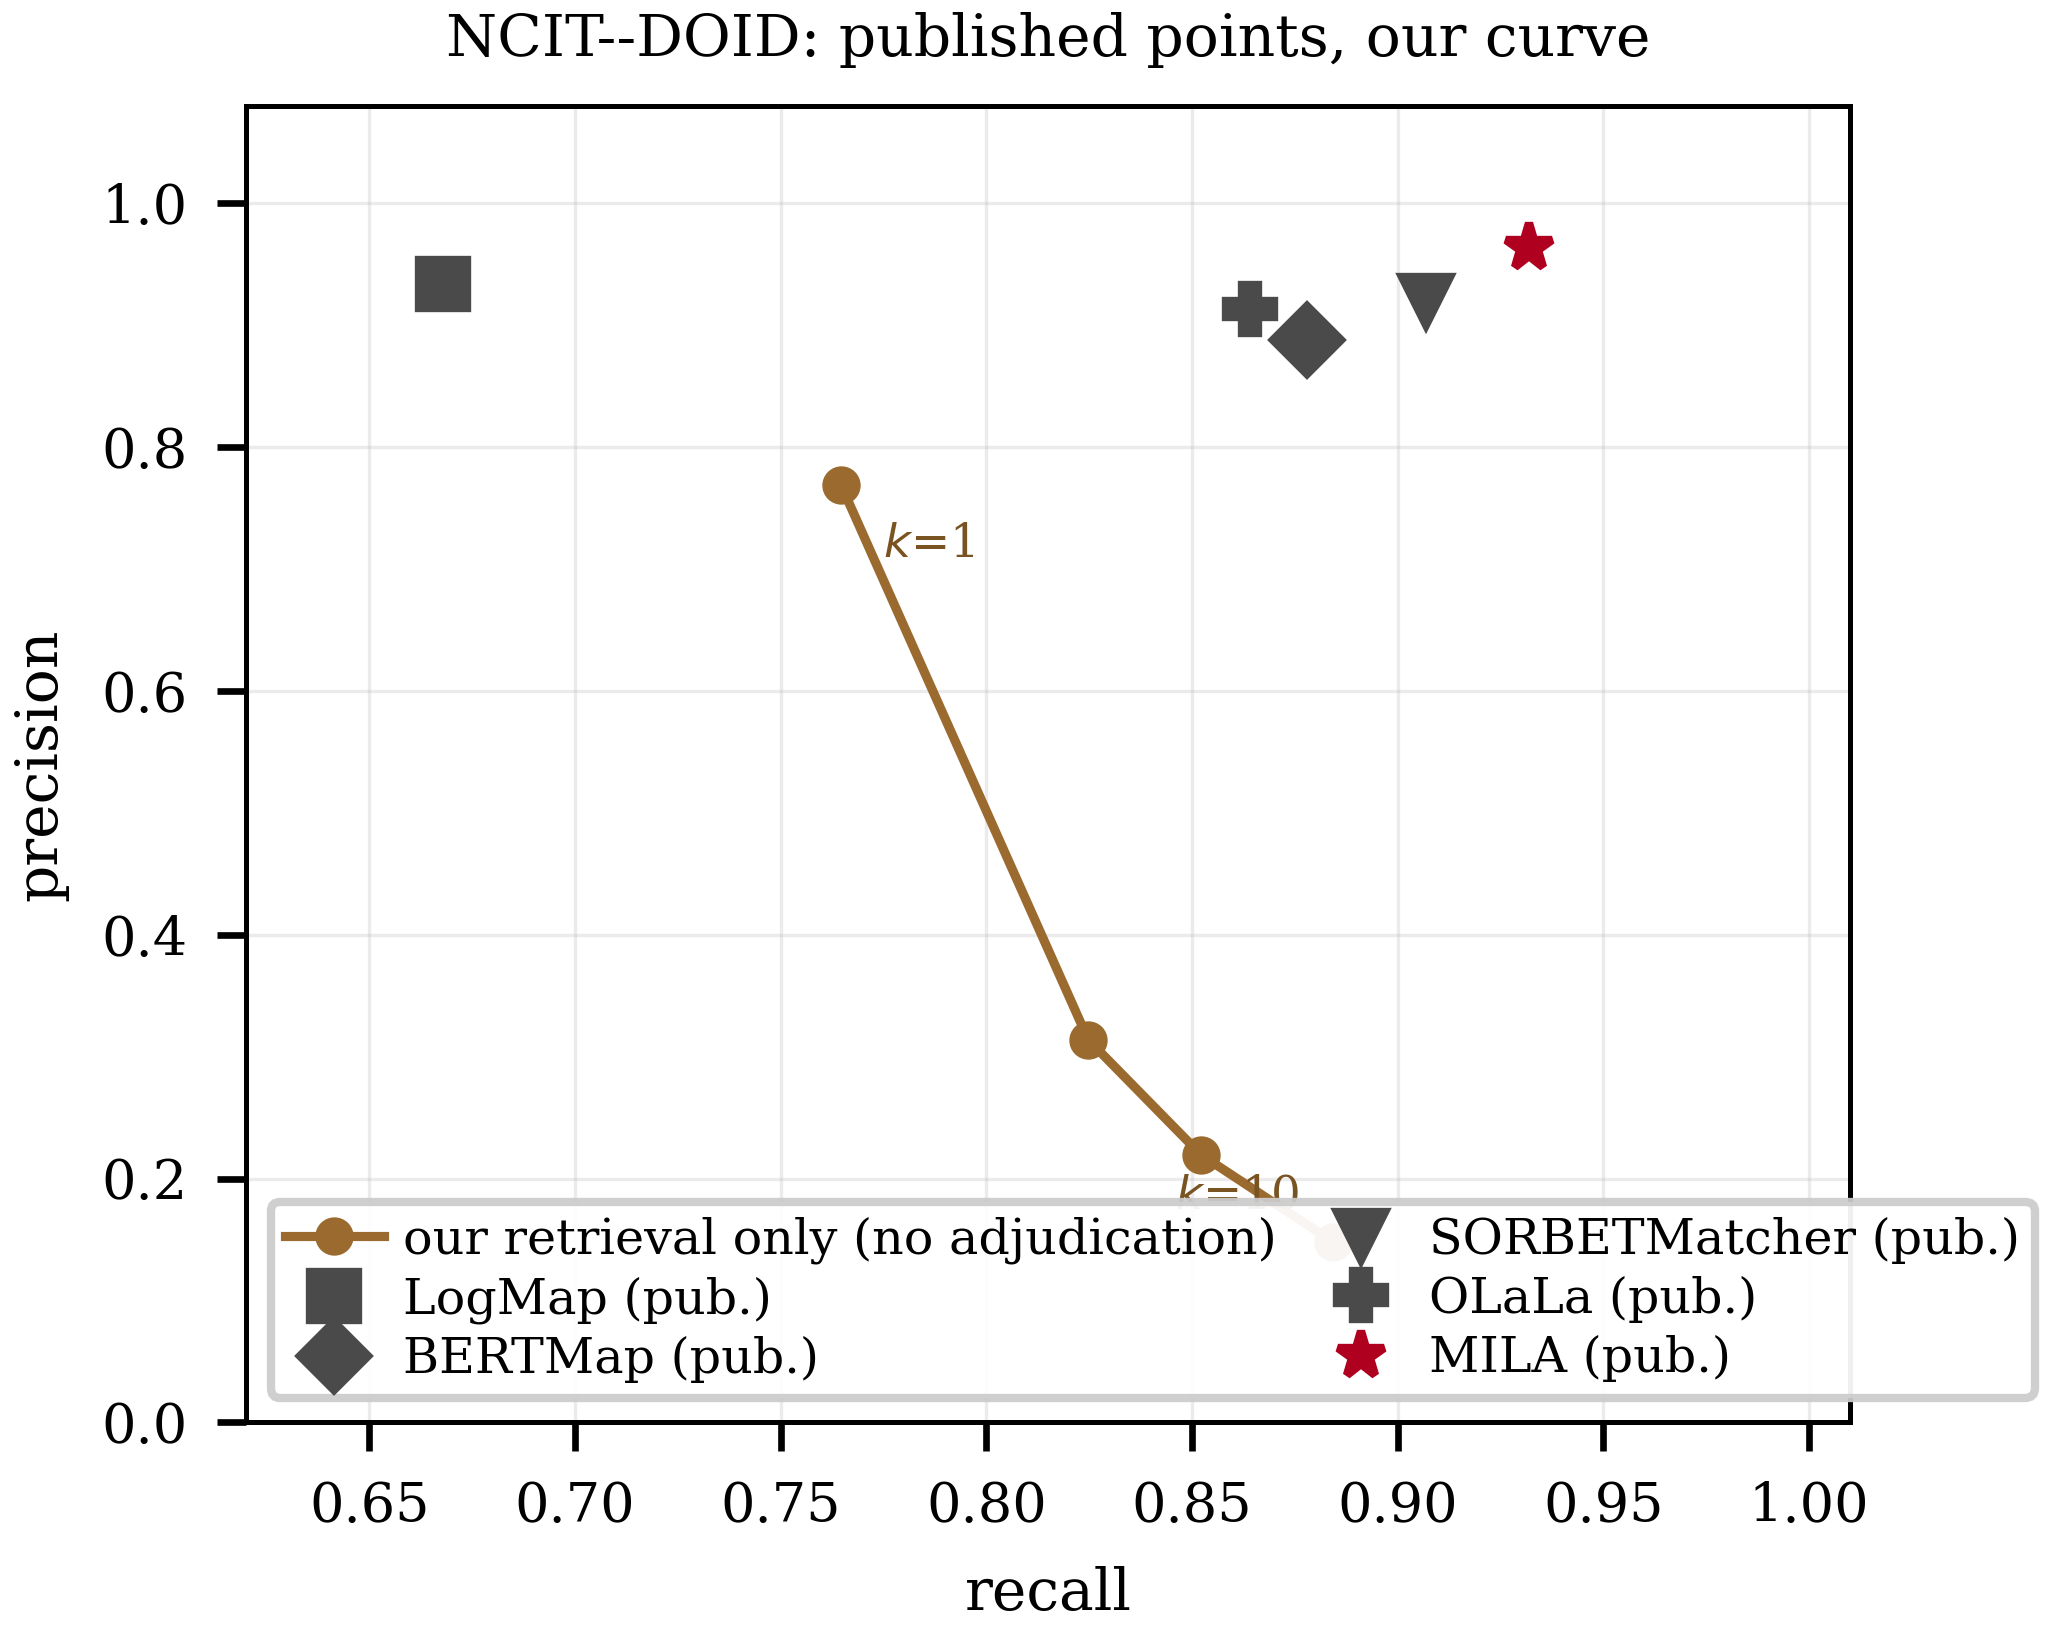
\includegraphics[width=\columnwidth]{figs/fig_pr_plane.png}
\caption{NCIT--DOID in the precision--recall plane. Published systems report a single operating point each, because they commit to every mapping they emit; our retrieval stage traces a curve, since the number of candidates is a free parameter. The two are not directly comparable---the published markers include mapping refinement, and ours does not---and the figure is included to make a reporting point rather than a competitive one: a scalar precision hides where on the trade-off a system sits, and the published point is the least informative place to measure it.}
\label{fig:prplane}
\end{figure}

\textbf{(ii) T3 is not supported.} Union over the lexical generator raises recall by 0.004 on NCIT--DOID (0.884 to 0.888) and by 0.000 on OMIM--ORDO (0.753 to 0.753), while increasing the mean candidate set by 23\% and 45\% respectively. The neighbourhood-expansion generator is worse than useless on its own---it adds candidates that are structurally adjacent but semantically distinct---and in an unbounded variant it degenerates entirely on OMIM--ORDO, where expansion around a high-level ORDO anchor produced a mean of 4{,}581 candidates. We therefore record T3 as tested and not supported in the configuration available to us, and we do not claim that generator union is what makes M1 work.

\begin{figure}[t]
\centering
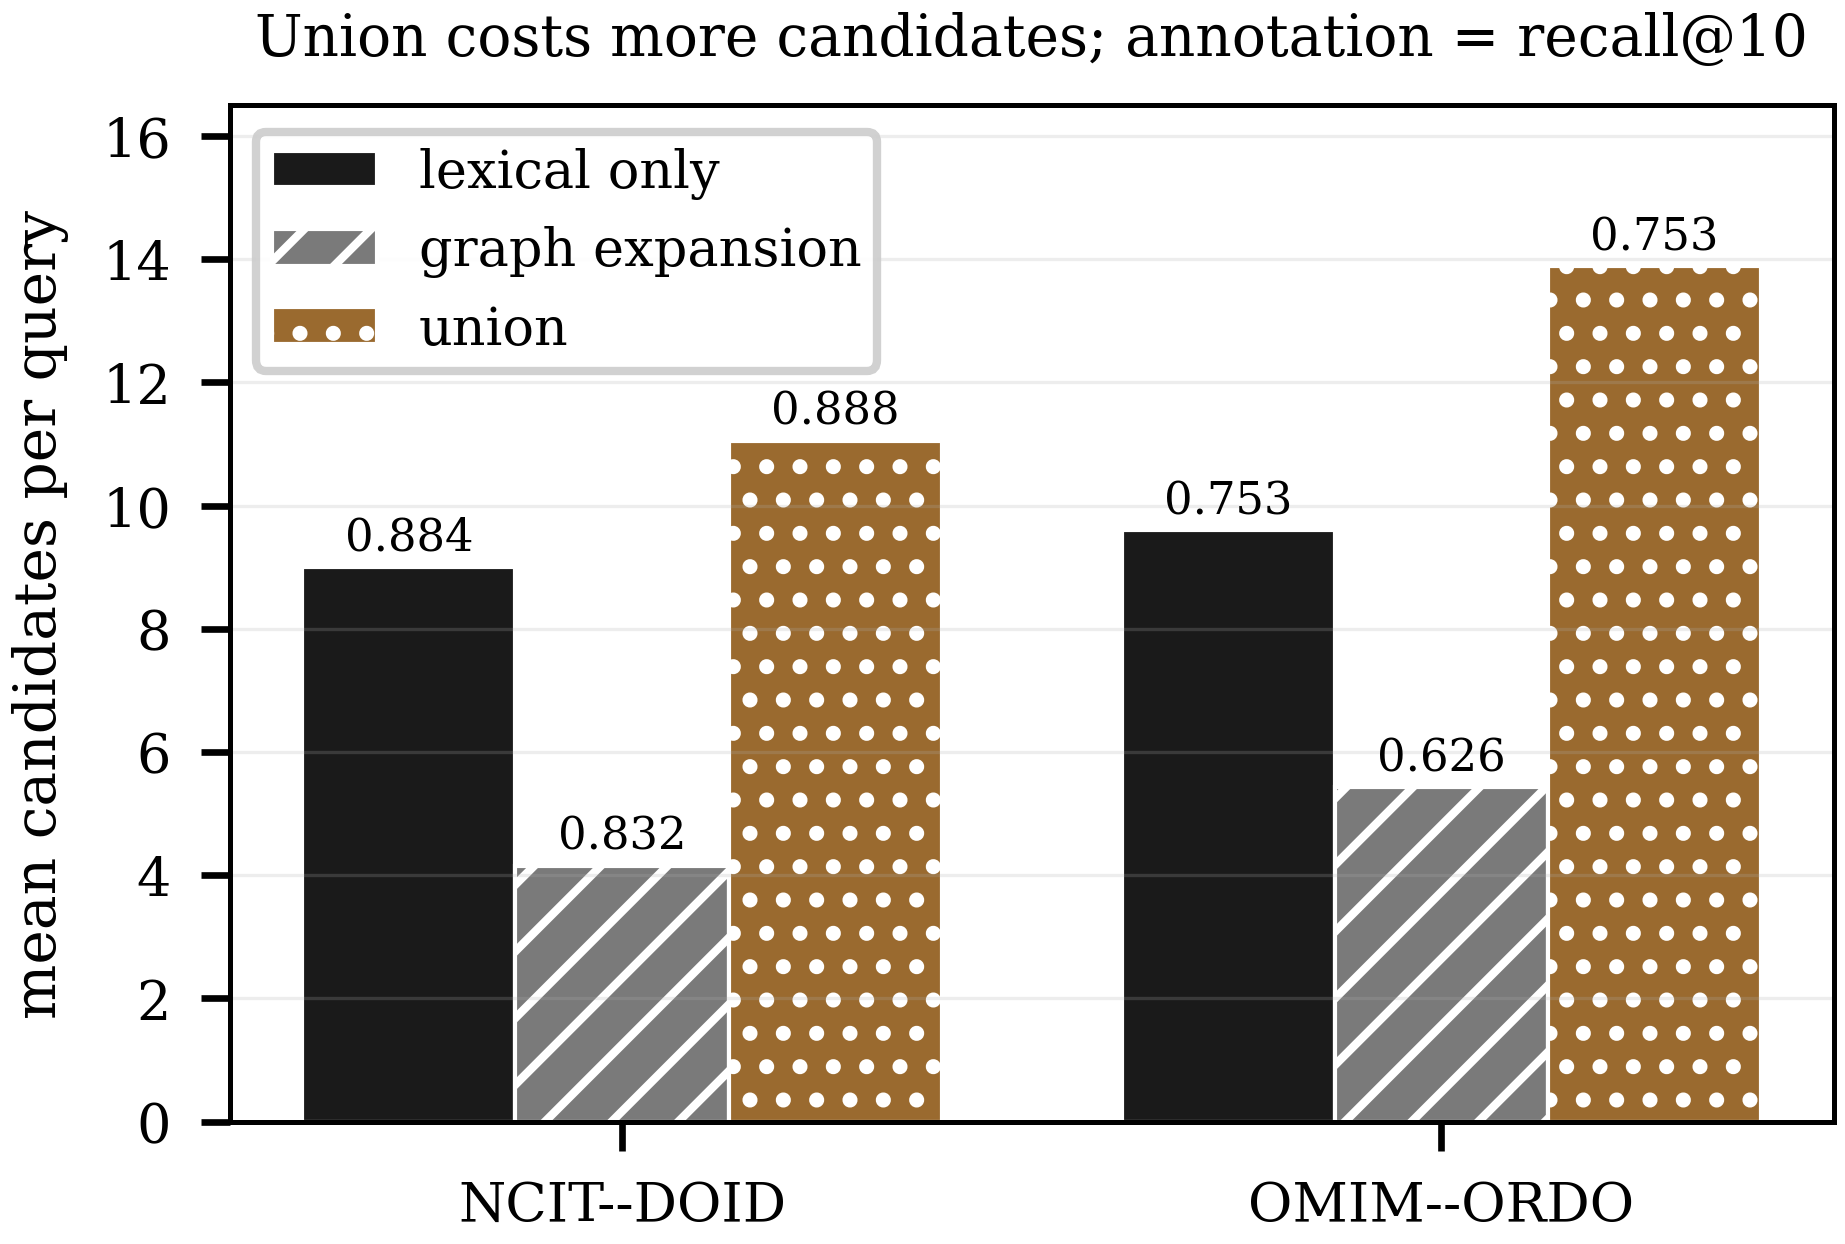
\includegraphics[width=\columnwidth]{figs/fig_cost.png}
\caption{The cost side of the same result. Bar height is the mean number of candidates each generator produces per query; the number above each bar is its recall at $k{=}10$. Union buys at most 0.004 recall over the lexical generator alone while producing 23\% (NCIT--DOID) and 45\% (OMIM--ORDO) more candidates, and every additional candidate is one the adjudicator must process. Under T1, where adjudicator calls are the scarce resource, this is a strictly bad trade.}
\label{fig:cost}
\end{figure}

Three qualifications bound how far this negative result should be read, and we state them in the order of how much they matter. First, the pilot exercises one of four generators; the generator the architecture most depends on for recall, dense retrieval over ontology labels, is absent. Our recall ceiling of 0.91 on NCIT--DOID at twenty candidates falls well short of the near-complete candidate recovery reported for full retrieve-then-prompt pipelines~\cite{b54}, which is consistent with a missing generator rather than with a property of the union. Second, the tasks are ontology-to-ontology alignments between curated terminologies with high lexical overlap. In the record-to-ontology setting that motivates the paper, the source is free clinical text, where lexical matching should degrade sharply and the case for complementary generators should be correspondingly stronger; a null result here does not transfer to MPRINT. Third, the graph generator we implemented expands without learned depth control, and its failure at high-level anchors is an argument for the bounded radius $r$ that M1 specifies rather than evidence against structural expansion in general. What the pilot does establish is narrower than any of these readings: on two curated alignment tasks, a well-tuned lexical generator is difficult to improve on with a naive second generator, and padding a candidate set is not free.

\section{Discussion}

The two-step pipeline and FedHarm agree on a division of labour and disagree on where the division ends. Both hold that generating candidates should be cheap and over-inclusive, and that validation should be expensive and precise. FedHarm adds three observations to that picture, each of which is a claim about which component of a system should own a decision.

\textbf{Symbolic and neural validation are complementary in the same way that lexical and dense retrieval are.} The source study established that two retrieval generators are complementary rather than interchangeable~\cite{b1}. We make the analogous claim one stage later: a reasoner and a language model fail differently. The reasoner is exactly right within its fragment and silent outside it; the LLM is broadly competent and locally unreliable, with failures concentrated on specificity and polarity, which are precisely the relations the reasoner settles. Ordering the reasoner first, and using it to supply the relation rather than the verdict, converts this complementarity from an opportunity into a pipeline invariant. It also explains the shape of the reported residual errors in~\cite{b1}: they are not random, they cluster in the relation structure, which is the signal a structure-aware stage captures.

\textbf{Uncertainty is not a metric but a control input.} The most consequential difference between a 92\%-accurate pipeline and a 92\%-accurate pipeline with a calibrated score and an abstention band is not accuracy; it is that the second can be deployed at a stated risk tolerance, because its errors are concentrated in a queue that a human can clear. The conformal construction in M4 is what makes the risk tolerance a property of the deployment rather than a hope about the model. It also changes the economics: expert time is allocated to the residual, and the residual shrinks as the registry fills.

\textbf{Reuse requires an artifact.} The source study's diagnosis of why federated workflows are rarely reusable---that they are built around a priori knowledge of the participating datasets---applies most sharply to harmonization, which is the one part of the workflow that is genuinely transferable. Ontology mappings do not depend on patient outcomes, on model architecture, or on study design; they depend only on the source and target vocabularies. This makes harmonization unusually well suited to being accumulated in a shared artifact, and the registry is the architecture's way of insisting on it. The result is an inversion of the usual federated-learning cost curve: instead of paying harmonization cost once per site and once per study, the consortium pays it once.

\textbf{The field has a benchmark it is not using.} The ontology-alignment community has spent a decade building curated reference alignments and standardizing evaluation through OAEI~\cite{b55}, and its published results are directly relevant to harmonization---most sharply the finding that retrieval reaches near-complete recall while prompting destroys a large fraction of it~\cite{b54}. Yet the harmonization systems we surveyed evaluate against a single expert on a bespoke dataset, and the alignment systems never touch patient-derived text or a federation constraint. The cost of this separation is that neither literature can falsify the other. Many of our own claims---that a symbolic stage recovers what adjudication loses, that calibration converts a model score into a deployable bound---are testable on Bio-ML today, at a fraction of the cost of a prospective multi-site study, and we have written the protocol to run there first for that reason. We regard the reuse of alignment benchmarks by harmonization work, and of patient-derived text by alignment work, as the cheapest available improvement to the field's evidentiary standard.

\textbf{What stays the same.} The architecture is ontology-agnostic: MONDO and HPO appear in the protocol because they appear in the reference setting, but nothing in M1--M4 references a particular vocabulary, and cross-reference pivoting is configured by supplying a cross-reference table rather than by changing code. It is also prompt-configurable, inheriting the property the source authors identified as the source pipeline's main design virtue. FedHarm changes what surrounds the prompt, not whether the prompt is the interface.

\section{Limitations and Threats to Validity}

\textit{Limited empirical coverage.} This paper specifies an architecture, proves properties of it, and defines a protocol for evaluating it. We execute one component: the retrieval pilot of Section~\ref{sec:pilot}, which covers one of M1's four generators on two of the five Bio-ML tasks. It is our only measurement. Tables~\ref{tab:oaei} and~\ref{tab:reported} reproduce numbers published by other systems and attribute each to its source, and the first block of Table~\ref{tab:results} does the same for the two baselines---we ran none of those experiments. Every cell of Table~\ref{tab:results} in the rows describing FedHarm is empty and marked as such, because adjudication, calibration, and the registry cannot be exercised without a language model. The propositions are conditional on their stated assumptions---reasoner soundness, exchangeability, accept-only retention, constant-size attestations---and the assumptions are the first thing an evaluation should attempt to violate.

\textit{Anchor dependence.} As noted above, M2's losslessness is relative to the anchor. On unannotated records the anchor is estimated, and the strength of Proposition~\ref{prop:prefilter} degrades with anchor error. Reporting anchor accuracy as a first-class metric, rather than as a preprocessing detail, is a requirement of the protocol and not an option.

\textit{Guarantee transfer across sites.} The conformal guarantee is distribution-free but not assumption-free: it needs exchangeability. A heterogeneous consortium breaks this, and the honest reading of M4 in that setting is a per-site guarantee with a cross-site diagnostic, not a global one.

\textit{Calibration data.} M4 requires labeled calibration data at each site, which reintroduces the annotation burden the architecture is meant to reduce. Our design keeps the calibration set small and treats it as a fixed one-off cost amortized over the registry's lifetime, but for a site joining at the end of a study the amortization is weak.

\textit{Registry governance.} A shared mapping artifact is a governance object as much as a technical one: who may attest, who may revoke, what the support threshold is, and how disputes are resolved are policy questions the architecture constrains but does not settle. Proposition~\ref{prop:registry} relies on accept-only retention, and any revocation policy trades monotonicity for correctness. We regard this as the most important open problem the design raises.

\textit{Scope of the reference setting.} The protocol is instantiated on the MONDO/HPO mapping task, and while the architecture is vocabulary-agnostic in principle, the strength of structural pre-filtering depends on how much of the target ontology is expressible in a tractable description-logic fragment. Ontologies with sparse axioms will yield more $\sim$ labels and push more work onto M3.

\section{Conclusion}

Federated learning without harmonization aggregates incomparable models. The two-step pipeline of~\cite{b1} demonstrated that harmonization can be largely automated, and its central insight---retrieval buys recall, validation buys precision---is one we adopt rather than revise. We have argued that the architecture around that insight can be rearranged so that validation is a stack rather than a step, decisions are committed under a calibrated risk bound rather than asserted, records are processed inside the trust boundary rather than through an API, and confirmed mappings are retained rather than discarded. The resulting architecture, FedHarm, adds an ontology-graph verifier ahead of the language model, a typed and evidence-citing adjudicator in its place, a conformal abstention rule after it, and a differentially private federated registry that closes the loop and makes harmonization cumulative across rounds and sites. We proved that the structural stage is lossless for the acceptance relation, that the abstention rule yields a finite-sample bound on selective risk, that registry coverage is monotone under accept-only retention, and that boundary communication is independent of local dataset size. What remains is the measurement we have only specified: a risk--coverage evaluation across sites, against a panel of experts, on the reference task and one further vocabulary pair, with the ablations of Section~\ref{sec:protocol}. The claim we are willing to defend is architectural---that reliable clinical harmonization requires the verification stack, the uncertainty control, and the retained artifact, and that a two-step pipeline, however well tuned, supplies only the middle of those three.

\begin{thebibliography}{00}

\bibitem{b1} N. Kokash, L. Wang, T. H. Gillespie, A. S. Z. Belloum, P. Grosso, S. Quinney, L. Li, and B. de Bono, ``Ontology- and LLM-based data harmonization for federated learning in healthcare,'' \emph{Frontiers in Digital Health}, vol. 8, art. 1756555, 2026, doi: 10.3389/fdgth.2026.1756555.

\bibitem{b2} P. Kairouz, H. B. McMahan, B. Avent, A. Bellet, M. Bennis, A. N. Bhagoji, et al., ``Advances and open problems in federated learning,'' \emph{Foundations and Trends in Machine Learning}, vol. 14, no. 1--2, pp. 1--210, 2021.

\bibitem{b3} H. B. McMahan, E. Moore, D. Ramage, S. Hampson, and B. A. y Arcas, ``Communication-efficient learning of deep networks from decentralized data,'' in \emph{Proc. AISTATS}, 2017, pp. 1273--1282.

\bibitem{b4} T. Li, A. K. Sahu, A. Talwalkar, and V. Smith, ``Federated learning: Challenges, methods, and future directions,'' \emph{IEEE Signal Processing Magazine}, vol. 37, no. 3, pp. 50--60, 2020.

\bibitem{b5} N. Rieke, J. Hancox, W. Li, F. Milletari, H. R. Roth, S. Albarqouni, et al., ``The future of digital health with federated learning,'' \emph{npj Digital Medicine}, vol. 3, art. 119, 2020.

\bibitem{b6} F. Zhang, D. Zhai, G. Bai, J. Jiang, Q. Ye, X. Ji, et al., ``Towards fairness-aware and privacy-preserving enhanced collaborative learning for healthcare,'' \emph{Nature Communications}, vol. 16, art. 2852, 2025.

\bibitem{b7} K. Donnelly, ``SNOMED-CT: The advanced terminology and coding system for eHealth,'' \emph{Studies in Health Technology and Informatics}, vol. 121, pp. 279--290, 2006.

\bibitem{b8} World Health Organization, \emph{International Statistical Classification of Diseases and Related Health Problems, 10th Revision (ICD-10)}. Geneva: WHO, 2004.

\bibitem{b9} N. A. Vasilevsky, N. A. Matentzoglu, S. Toro, J. E. Flack, H. Hegde, D. R. Unni, et al., ``Mondo: Unifying disease ontologies representation through logical definitions,'' \emph{Database}, vol. 2022, art. baac041, 2022.

\bibitem{b10} S. K\"ohler, M. Gargano, N. Matentzoglu, L. C. Carmody, D. Lewis-Smith, N. A. Vasilevsky, et al., ``The Human Phenotype Ontology in 2021,'' \emph{Nucleic Acids Research}, vol. 49, no. D1, pp. D1207--D1217, 2021.

\bibitem{b11} J. J. Cimino, ``Desiderata for controlled medical vocabularies in the twenty-first century,'' \emph{Methods of Information in Medicine}, vol. 37, no. 4--5, pp. 394--403, 1998.

\bibitem{b12} O. Bodenreider, ``The Unified Medical Language System (UMLS): Integrating biomedical terminology,'' \emph{Nucleic Acids Research}, vol. 32, no. suppl\_1, pp. D267--D270, 2004.

\bibitem{b13} G. Hripcsak, J. D. Duke, N. H. Shah, C. G. Reich, V. Huser, M. J. Schuemie, et al., ``Observational Health Data Sciences and Informatics (OHDSI): Opportunities for observational researchers,'' \emph{Studies in Health Technology and Informatics}, vol. 216, pp. 574--578, 2015.

\bibitem{b14} M. A. Haendel, C. G. Chute, and P. N. Robinson, ``Classification, ontology, and precision medicine,'' \emph{New England Journal of Medicine}, vol. 379, no. 15, pp. 1452--1462, 2018.

\bibitem{b15} P. Lewis, E. Perez, A. Piktus, F. Petroni, V. Karpukhin, N. Goyal, et al., ``Retrieval-augmented generation for knowledge-intensive NLP tasks,'' in \emph{Proc. NeurIPS}, 2020, pp. 9459--9474.

\bibitem{b16} V. Karpukhin, B. O\u{g}uz, S. Min, P. Lewis, L. Wu, S. Edunov, D. Chen, and W. Yih, ``Dense passage retrieval for open-domain question answering,'' in \emph{Proc. EMNLP}, 2020, pp. 6769--6781.

\bibitem{b17} S. Robertson and H. Zaragoza, ``The probabilistic relevance framework: BM25 and beyond,'' \emph{Foundations and Trends in Information Retrieval}, vol. 3, no. 4, pp. 333--389, 2009.

\bibitem{b18} N. Reimers and I. Gurevych, ``Sentence-BERT: Sentence embeddings using Siamese BERT-networks,'' in \emph{Proc. EMNLP-IJCNLP}, 2019, pp. 3982--3992.

\bibitem{b19} C. Guo, G. Pleiss, Y. Sun, and K. Q. Weinberger, ``On calibration of modern neural networks,'' in \emph{Proc. ICML}, 2017, pp. 1321--1330.

\bibitem{b20} Y. Geifman and R. El-Yaniv, ``Selective classification for deep neural networks,'' in \emph{Proc. NeurIPS}, 2017, pp. 4878--4887.

\bibitem{b21} C. K. Chow, ``On optimum recognition error and reject tradeoff,'' \emph{IEEE Transactions on Information Theory}, vol. 16, no. 1, pp. 41--46, 1970.

\bibitem{b22} A. N. Angelopoulos, S. Bates, A. Fisch, L. Lei, and T. Schuster, ``Conformal risk control,'' in \emph{Proc. ICLR}, 2024.

\bibitem{b23} V. Vovk, A. Gammerman, and G. Shafer, \emph{Algorithmic Learning in a Random World}. New York: Springer, 2005.

\bibitem{b24} M. Abadi, A. Chu, I. Goodfellow, H. B. McMahan, I. Mironov, K. Talwar, and L. Zhang, ``Deep learning with differential privacy,'' in \emph{Proc. ACM CCS}, 2016, pp. 308--318.

\bibitem{b25} H. B. McMahan, D. Ramage, K. Talwar, and L. Zhang, ``Learning differentially private recurrent language models,'' in \emph{Proc. ICLR}, 2018.

\bibitem{b26} K. Bonawitz, V. Ivanov, B. Kreuter, A. Marcedone, H. B. McMahan, S. Patel, D. Ramage, A. Segal, and K. Seth, ``Practical secure aggregation for privacy-preserving machine learning,'' in \emph{Proc. ACM CCS}, 2017, pp. 1175--1191.

\bibitem{b27} T. Li, A. K. Sahu, M. Zaheer, M. Sanjabi, A. Talwalkar, and V. Smith, ``Federated optimization in heterogeneous networks,'' in \emph{Proc. MLSys}, 2020.

\bibitem{b28} S. Kadavath, T. Conerly, A. Askell, T. Henighan, D. Drain, E. Perez, et al., ``Language models (mostly) know what they know,'' arXiv:2207.05221, 2022.

\bibitem{b29} J. Euzenat and P. Shvaiko, \emph{Ontology Matching}, 2nd ed. Berlin: Springer, 2013.

\bibitem{b30} B. Glimm, I. Horrocks, B. Motik, G. Stoilos, and Z. Wang, ``HermiT: An OWL 2 reasoner,'' \emph{Journal of Automated Reasoning}, vol. 53, no. 3, pp. 245--269, 2014.

\bibitem{b31} Y. Kazakov, M. Kr\"otzsch, and F. Siman\v{c}\'ik, ``The incredible ELK: From polynomial procedures to efficient reasoning with $\mathcal{EL}$ ontologies,'' \emph{Journal of Automated Reasoning}, vol. 53, no. 1, pp. 1--61, 2014.

\bibitem{b32} B. C. Grau, I. Horrocks, B. Motik, B. Parsia, P. Patel-Schneider, and U. Sattler, ``OWL 2: The next step for OWL,'' \emph{Journal of Web Semantics}, vol. 6, no. 4, pp. 309--322, 2008.

\bibitem{b33} O. Valkering, R. Cushing, and A. Belloum, ``Brane: A framework for programmable orchestration of multi-site applications,'' in \emph{Proc. IEEE eScience}, 2021, pp. 277--282.

\bibitem{b34} A. Moncada-Torres, F. Martin, M. Sieswerda, J. van Soest, and G. Geleijnse, ``VANTAGE6: An open source privacy-preserving federated learning infrastructure for secure insight exchange,'' in \emph{Proc. AMIA Annual Symposium}, 2021, pp. 870--877.

\bibitem{b35} J. Alsayed Kassem, C. Allaart, S. Amiri, M. Kebede, T. M\"uller, R. Turner, et al., ``Building a digital health twin for personalized intervention: The EPI project,'' in \emph{Open Access Series in Informatics (OASIcs)}, vol. 124, 2024, pp. 2:1--2:18.

\bibitem{b36} C. Chen, X. Feng, Y. Li, L. Lyu, J. Zhou, X. Zheng, et al., ``Integration of large language models and federated learning,'' \emph{Patterns}, vol. 5, art. 101098, 2024.

\bibitem{b37} S. K. Quinney, R. R. Bies, S. J. Grannis, C. W. Bartlett, E. Mendonca, C. M. Rogerson, et al., ``The MPRINT hub data, model, knowledge and research coordination center: Bridging the gap in maternal--pediatric therapeutics research through data integration and pharmacometrics,'' \emph{Pharmacotherapy}, vol. 43, no. 12, pp. e14--e25, 2023.

\bibitem{b38} M. Stonebraker and I. F. Ilyas, ``Data integration: The current status and the way forward,'' \emph{IEEE Data Engineering Bulletin}, vol. 41, no. 2, pp. 3--9, 2018.

\bibitem{b39} A. Santos, A. Garcia, E. Strubell, T. Rekatsinas, F. T. Li, and R. B. Altman, ``Interactive data harmonization with LLM agents,'' arXiv:2502.07132, 2025.

\bibitem{b40} J. Matos, M. C. Hughes, L. H. Lehman, P. Szolovits, and I. Y. Chen, ``EHRmonize: A framework for medical concept abstraction from electronic health records using large language models,'' arXiv:2407.00242, 2024.

\bibitem{b41} Y. Li, Z. Wang, Y. Wang, L. Rasmy, P. Nguyen, Y. Wang, et al., ``Enhancing health data interoperability with large language models: A FHIR study,'' arXiv:2310.12989, 2023.

\bibitem{b42} Y. Nan, J. Del Ser, S. Walsh, C. Sch\"onlieb, M. Roberts, I. Selby, et al., ``Data harmonisation for information fusion in digital healthcare: A state-of-the-art systematic review, meta-analysis and future research directions,'' \emph{Information Fusion}, vol. 82, pp. 99--122, 2022.

\bibitem{b43} B. Schmidt, C. Colvin, A. Hohlfeld, and N. Leon, ``Definitions, components and processes of data harmonisation in healthcare: A scoping review,'' \emph{BMC Medical Informatics and Decision Making}, vol. 20, art. 222, 2020.

\bibitem{b44} I. Jahan, M. T. R. Laskar, C. Peng, and J. X. Huang, ``A comprehensive evaluation of large language models on benchmark biomedical text processing tasks,'' \emph{Computers in Biology and Medicine}, vol. 171, art. 108189, 2024.

\bibitem{b45} L. Wang, Z. Wan, C. Ni, Q. Song, Y. Li, E. Clayton, et al., ``Applications and concerns of ChatGPT and other conversational large language models in health care: Systematic review,'' \emph{Journal of Medical Internet Research}, vol. 26, art. e22769, 2024.

\bibitem{b46} HL7 International, \emph{FHIR R4: Fast Healthcare Interoperability Resources Specification}. Ann Arbor, MI: HL7, 2019.

\bibitem{b47} B. Zadrozny and C. Elkan, ``Transforming classifier scores into accurate multiclass probability estimates,'' in \emph{Proc. ACM SIGKDD}, 2002, pp. 694--699.

\bibitem{b48} N. Kokash, L. Wang, T. H. Gillespie, A. S. Z. Belloum, P. Grosso, S. Quinney, L. Li, and B. de Bono, ``Ontology- and LLM-based data harmonization for federated learning in healthcare,'' arXiv:2505.20020, 2025.

\bibitem{b49} H. Abbasizanjani, F. Torabi, and E. A. Bedston, ``Harmonising electronic health records for reproducible research: Challenges, solutions and recommendations from a UK-wide COVID-19 research collaboration,'' \emph{BMC Medical Informatics and Decision Making}, vol. 23, art. 8, 2023.

\bibitem{b50} A. N. Angelopoulos and S. Bates, ``A gentle introduction to conformal prediction and distribution-free uncertainty quantification,'' arXiv:2107.07511, 2021.

\bibitem{b51} P. Blanchard, E. M. El Mhamdi, R. Guerraoui, and J. Stainer, ``Machine learning with adversaries: Byzantine tolerant gradient descent,'' in \emph{Proc. NeurIPS}, 2017, pp. 119--129.

\bibitem{b52} Y. Jin and E. J. Cand\`es, ``Selection by prediction with conformal p-values,'' \emph{Journal of Machine Learning Research}, vol. 24, no. 244, pp. 1--41, 2023.

\bibitem{b53} Y. Benjamini and Y. Hochberg, ``Controlling the false discovery rate: A practical and powerful approach to multiple testing,'' \emph{Journal of the Royal Statistical Society: Series B}, vol. 57, no. 1, pp. 289--300, 1995.

\bibitem{b54} M. Taboada, D. Martinez, M. Arideh, and R. Mosquera, ``Ontology matching with large language models and prioritized depth-first search,'' arXiv:2501.11441, 2025.

\bibitem{b55} Y. He, J. Chen, H. Dong, E. Jim\'enez-Ruiz, A. Hadian, and I. Horrocks, ``Machine learning-friendly biomedical datasets for equivalence and subsumption ontology matching,'' in \emph{Proc. ISWC}, 2022, pp. 575--591.

\bibitem{b56} H. B. Giglou, J. D'Souza, and S. Auer, ``LLMs4OM: Matching ontologies with large language models,'' arXiv:2404.10317, 2024.

\bibitem{b57} S. Hertling and H. Paulheim, ``OLaLa: Ontology matching with large language models,'' in \emph{Proc. 12th Knowledge Capture Conference}, 2023, pp. 131--139.

\bibitem{b58} Y. He, J. Chen, D. Antonyrajah, and I. Horrocks, ``BERTMap: A BERT-based ontology alignment system,'' in \emph{Proc. AAAI}, vol. 36, 2022, pp. 5684--5691.

\bibitem{b59} E. Jim\'enez-Ruiz and B. Cuenca Grau, ``LogMap: Logic-based and scalable ontology matching,'' in \emph{Proc. ISWC}, 2011, pp. 273--288.

\bibitem{b60} L. Ferraz, P. G. Cotovio, and C. Pesquita, ``Can language models align biomedical ontologies? Evaluating retrieval-augmented prompt strategies in Bio-ML,'' in \emph{Proc. SeWebMeDa}, CEUR-WS Vol. 4001, 2025.

\bibitem{b61} F. Gosselin and A. Zouaq, ``SORBET: A Siamese network for ontology embeddings using a distance-based regression loss and BERT,'' in \emph{Proc. ISWC}, 2023, pp. 561--578.

\bibitem{b62} Office of the National Coordinator for Health Information Technology, \emph{United States Core Data for Interoperability (USCDI), Version 3}. Washington, DC: ONC, 2023.

\end{thebibliography}

\end{document}
